\documentclass[mathserif]{beamer}
%\documentclass{beamer}
\usetheme{Luebeck}
\usecolortheme{spruce}
\usecolortheme{rose}
\usepackage{amsmath,verbatim}
\usepackage{listings}
\usepackage[english]{babel}
%\usepackage{media9} % package for genuine embedding of movies
\usepackage{multimedia} % beamer package for calling external files and players
\setbeamercovered{transparent}

% media9 stuff for playing movies
%\newcommand{\includemovie}[3]{\includemedia[width=#1,height=#2,activate=pagevisible,deactivate=pageclose,addresource=#3,flashvars={src=#3 &autoPlay=true &loop=true &controlBarAutoHideTimeout=0 }]{}{VPlayer.swf}}

\newcommand{\trans}{\ensuremath{{}^\mathrm{T}}}
\newcommand{\eps}{\varepsilon}
\newcommand*{\approxdist}{\mathrel{\vcenter{\offinterlineskip
\vskip-.25ex\hbox{\hskip.55ex$\cdot$}\vskip-.25ex\hbox{$\sim$}
\vskip-.5ex\hbox{\hskip.55ex$\cdot$}}}}

\lstdefinelanguage{myR}
{
   language=R,
   otherkeywords={read.table, set.seed, head},
   deletekeywords={url,codes, t, dt, Call, formula,Q, R, on,by,hat,is,
col, set,start,end,deltat,zip},
   sensitive=true,
   breaklines=true,
   morecomment=[l]{\#},
   morestring=[b]",
   morestring=[b]',
   basicstyle =\ttfamily\small,
   keywordstyle=\bfseries,
   showtabs=false,
   showstringspaces=false,
   literate= {~}{$\sim$}{2},
   numberstyle=\sffamily\scriptsize,
   stepnumber=2
 }

\lstset{basicstyle=\ttfamily\color{blue}}

\begin{document}

\title{Scalable algorithms for Markov process parameter inference}
\author[Darren Wilkinson --- Banff, 12/11/18]{\textbf{\large Darren Wilkinson} \\
\url{@darrenjw}\\
\alert{\url{tinyurl.com/darrenjw}}\\
Newcastle University, U.K.\\ and\\
The Alan Turing Institute, U.K.}
\date{Connecting models and data in the life sciences\\BIRS, Banff, Alberta, Canada\\12th November 2018}

\frame{\titlepage}



\frame{
\frametitle{Overview}
\begin{itemize}
%\item Stochastic reaction networks: Modelling, simulation and inference
\item Stochastic reaction networks, stochastic simulation and partially observed Markov process (POMP) models
  \item Modularity: separating model representation from simulation algorithm
  \item Well-mixed versus reaction--diffusion
  \item Likelihood-free MCMC for POMP models: separating simulation from inference
    \item Likelihood-free PMMH pMCMC, ABC and ABC--SMC
%\item Likelihood-free (PMMH) pMCMC --- exact fully Bayesian joint inference for the model state and static parameters
%\item Efficient (PMMH) pMCMC for diffusion processes
%\item Efficient (PMMH) pMCMC for Markov jump processes
%\item (Adaptive) ABC(--SMC)
%\item Comparing pMCMC and ABC
  %\item Hybrid ABC/pMCMC approaches
\item Functional programming approaches for scalable scientific and statistical computing 
\end{itemize}
%Some joint work with \alert{Jamie Owen} and \alert{Colin Gillespie}
}

%\section{Modelling and simulation}

%\subsection{Well-mixed models}

\frame{
\frametitle{Example --- genetic auto-regulation}
%\includegraphics[width=12cm,clip=true]{figs/auto-reg}
\centerline{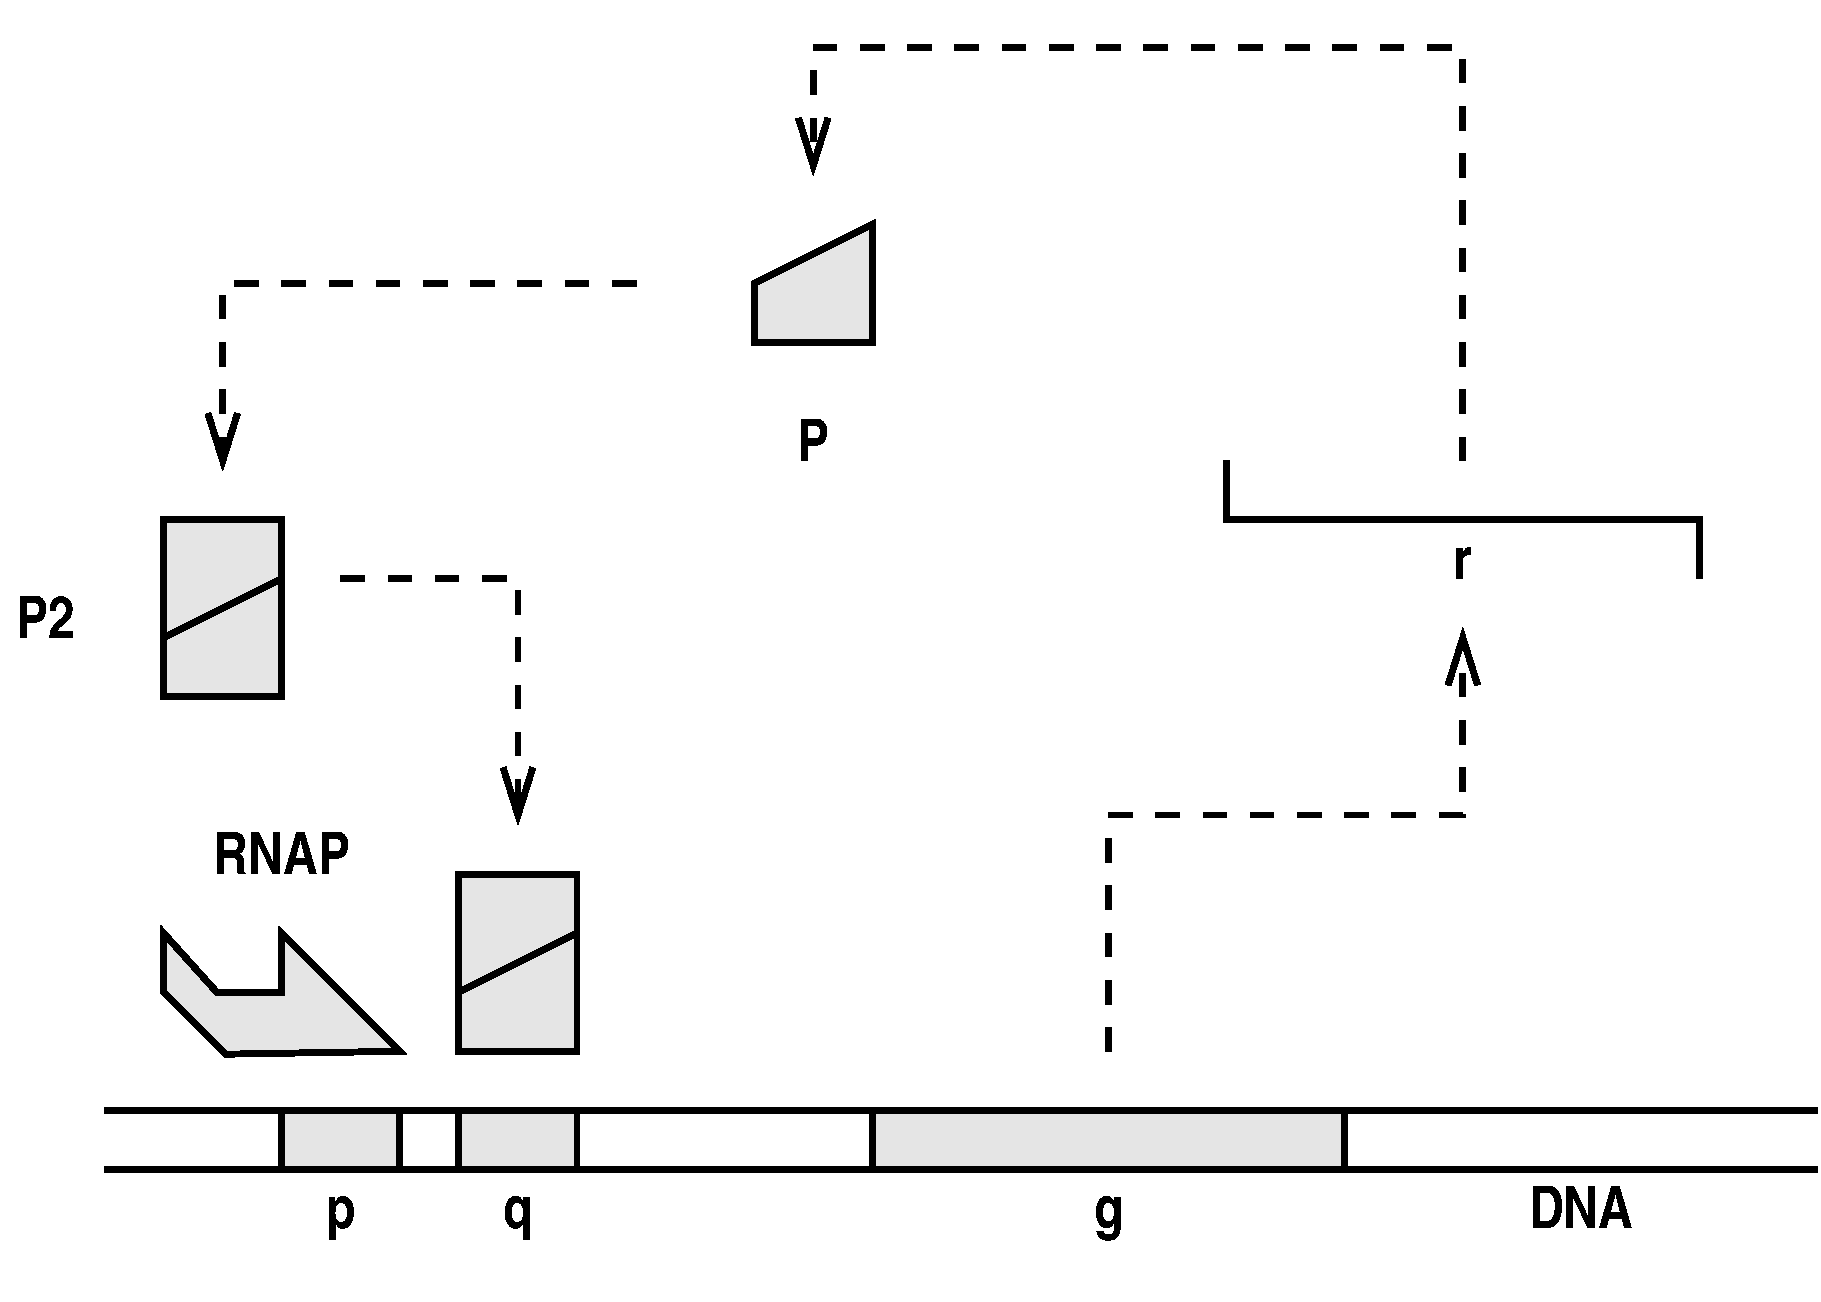
\includegraphics[width=8cm,clip=true]{figs/ch01-auto-reg}}
}




\frame{
\frametitle{Simulated realisation of the auto-regulatory network}
\centerline{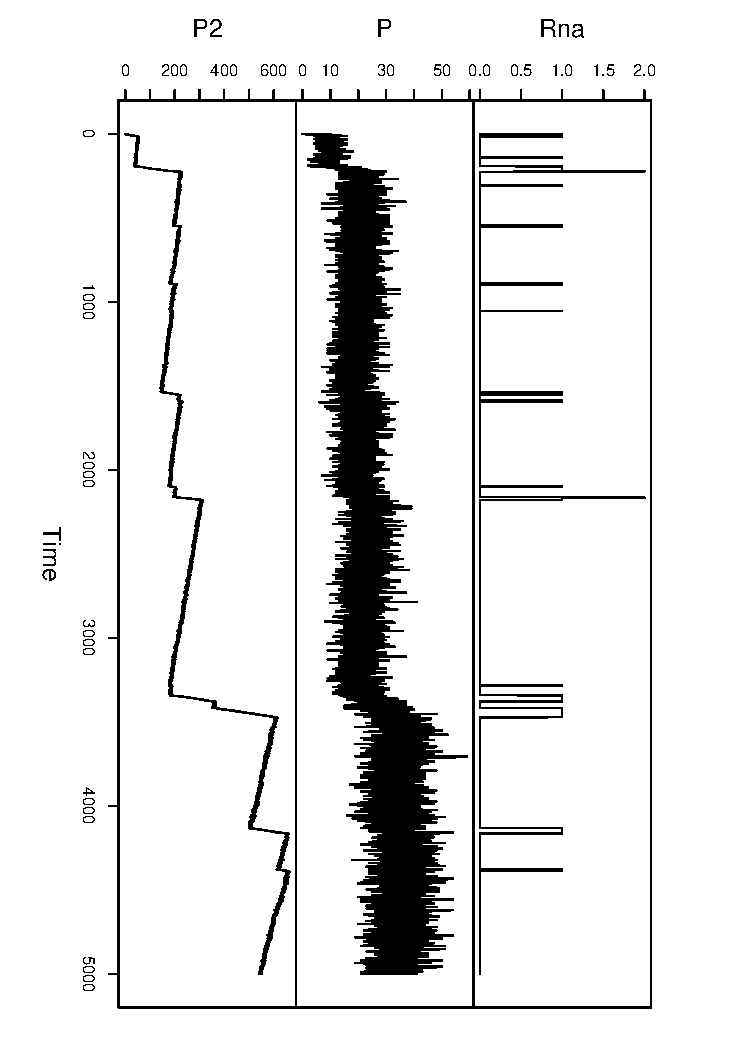
\includegraphics[height=9cm,clip=true,angle=90]{figs/ch07-ar-stochastic}}
}

\begin{comment}
  
\frame{
\frametitle{Multi-scale simulation issues}
\begin{itemize}
\item Although not a huge model, this is actually rather challenging, for both simulation and inference
\item Some species have very low copy number (predominantly zero or one), making the diffusion approximation unappealing, and some have fairly high copy number (several hundred)
\item The high and low copy-number species are tightly coupled, leading to very discrete bursty stochastic behaviour even in the high copy-number species
\item There are also two pairs of fast binding/unbinding reactions, making the problem difficult for time-stepping methods such as $\tau$-leaping
\item A rather sophisticated hybrid multi-scale algorithm would be required to simulate this process very accurately and very fast... 
\end{itemize}
}

\end{comment}

%\subsection{Modularity}

\frame{
\frametitle{Modularity: decoupling models from simulation algorithms}
\begin{itemize}
\item For forward modelling, there are clear and considerable benefits to \alert{separating} the \alert{representation} of the model from the algorithm used to \alert{simulate} realisations from it:
 \begin{itemize}
   \item There are numerous exact and approximate simulation algorithms, as well as algorithms for static model analysis --- by decoupling the models from the algorithms, it is easy to apply any algorithm to any model of interest --- improvements in simulation algorithms automatically apply to all models of interest
   \item \alert{Modifying} a model representation will typically be much easier than modifying an algorithm to simulate that model
   \item When assembling large models from smaller model components, it is often more straightforward to \alert{compose} model representations than associated simulation algorithms
 \end{itemize}
\item Few disadvantages: limit to flexibility of representation, slight inefficiencies, more sophisticated programming required
\end{itemize}
}



%%%%%%%%%%%%%%%%%%%


\frame{
\frametitle{Lotka--Volterra system}
Trivial (familiar) example from population dynamics, but here the
``reactions'' are elementary biochemical reactions taking place
inside a cell
%The running example through this talk will be a familiar example from population dynamics --- the Lotka--Volterra predator--prey system. We will regard it as a particular example of a broad class of nonlinear multivariate Markov jump processes known as \alert{stochastic kinetic models}
\begin{block}{Reactions}
\begin{align*}
X &\longrightarrow 2X \tag{prey reproduction}\\
X+Y &\longrightarrow 2Y \tag{prey-predator interaction}\\
Y &\longrightarrow \emptyset \tag{predator death}
\end{align*}
\end{block}
\begin{itemize}
\item $X$ -- Prey, $Y$ -- Predator
\item We can re-write this using matrix notation
% for the corresponding Petri net
\end{itemize}
}



\frame{
\frametitle{The Lotka-Volterra model}
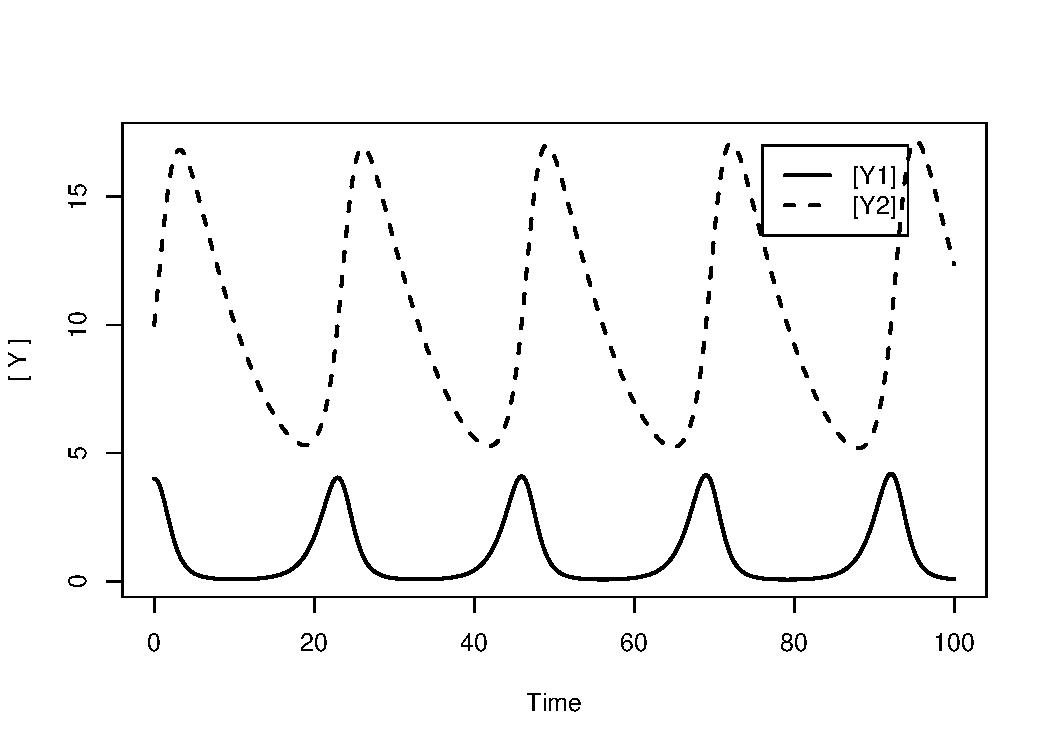
\includegraphics[width=5cm,clip=true]{ch06-lv-dynamics}
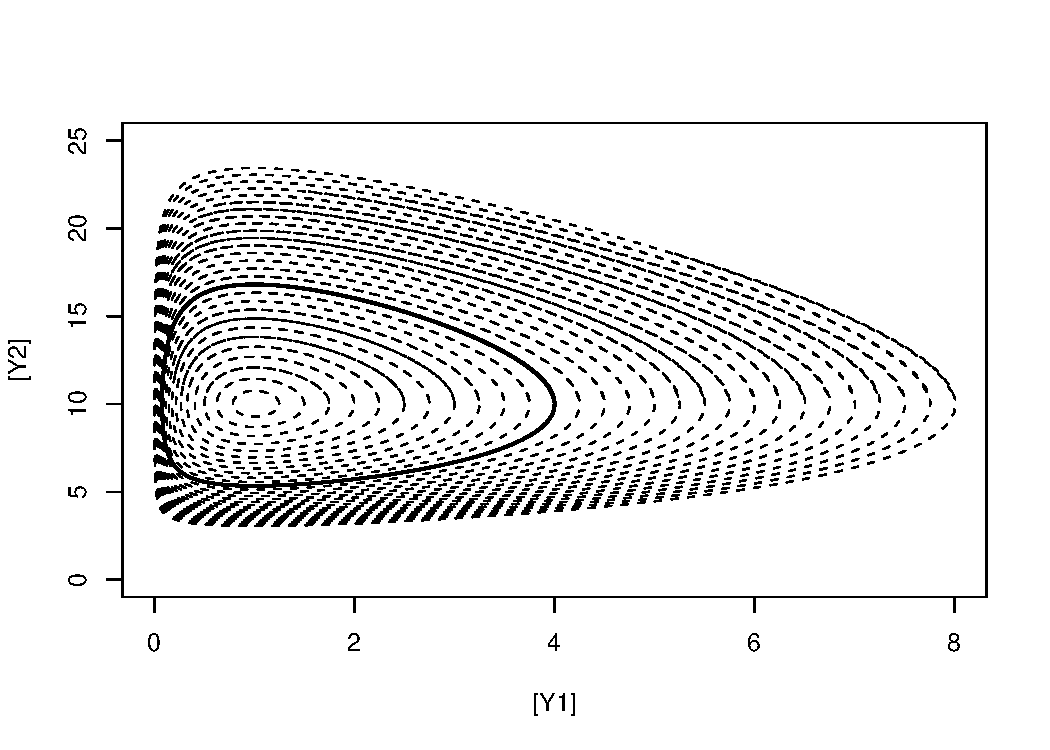
\includegraphics[width=5cm,clip=true]{ch06-lv-phase}
\\
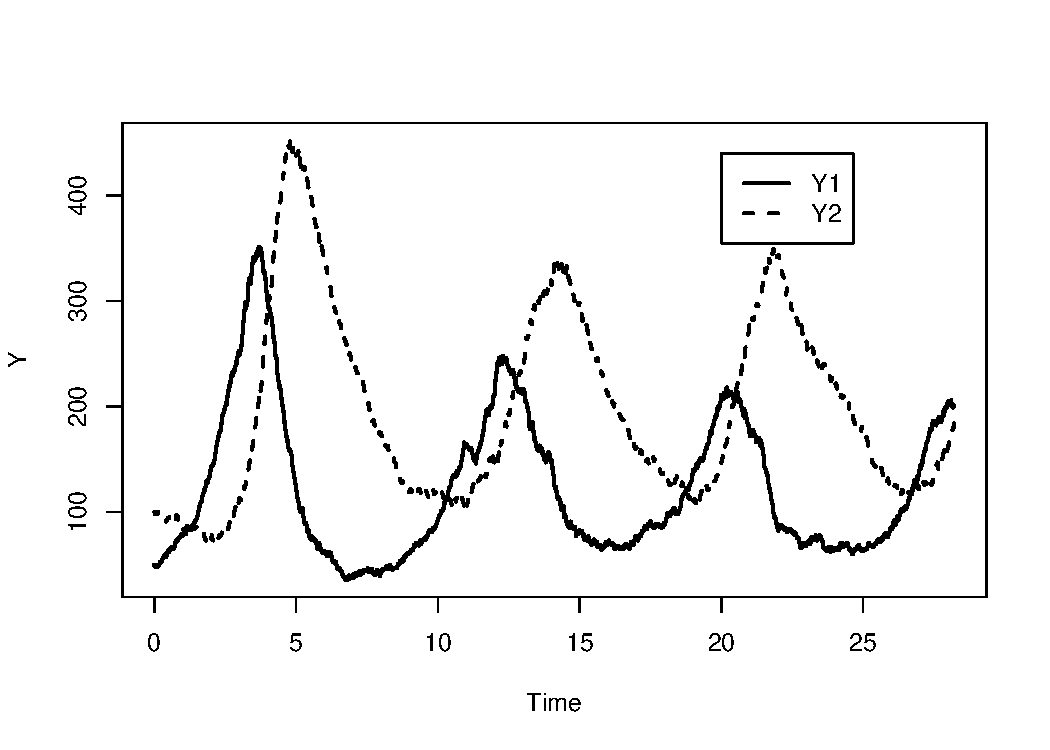
\includegraphics[width=5cm,clip=true]{ch06-stoch-lv}
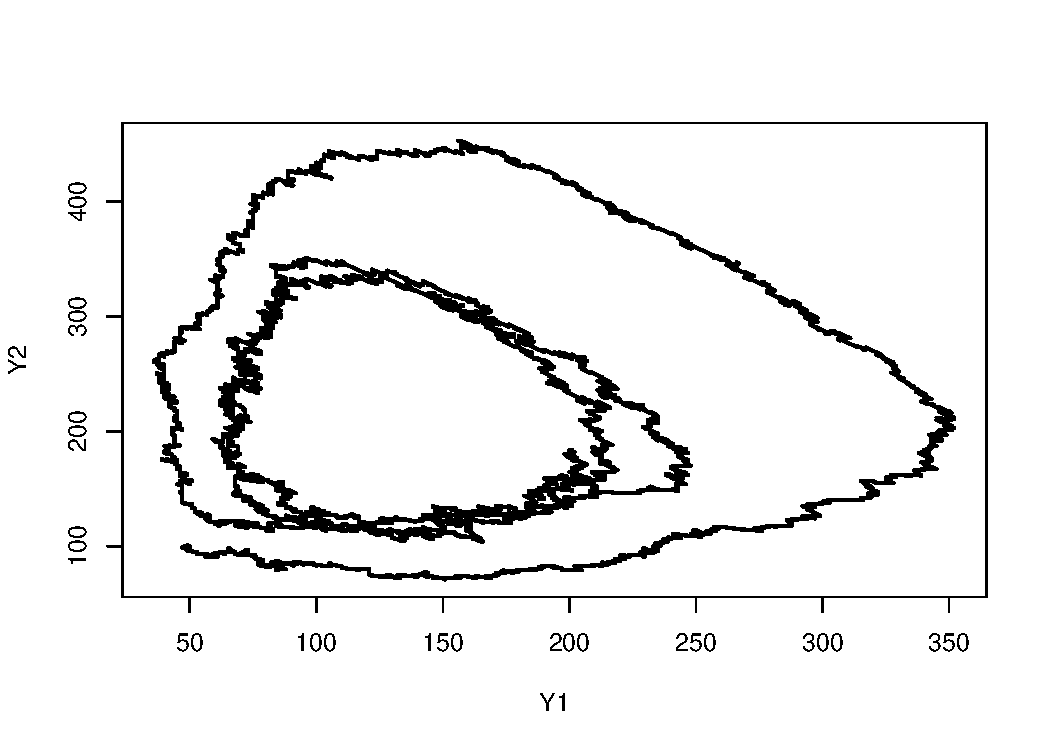
\includegraphics[width=5cm,clip=true]{ch06-stoch-lv-phase}
}

%\subsection{Spatially explicit models}

\frame{
\frametitle{The well-mixed assumption}
\begin{itemize}
\item The fundamental assumption underpinning the mass-action stochastic kinetic approach to modelling chemical reactions as a Markov jump process is that the hazard associated with any reaction event is \alert{constant}
\item It is this assumption of constant hazard which leads to exponential inter-arrival times of reaction events and all of the other algorithms commonly used for non-spatial modelling
\item However, it's pretty clear that molecules far apart will have a lower reaction hazard than molecules which are nearby
\item Mass-action kinetics assumes that molecular \alert{diffusion} is rapid relative to the time scales associated with the chemical \alert{reactions}
\item Evidence that this assumption is violated for many interesting intra-cellular processes
\end{itemize}
}

\begin{comment}

\frame{
\frametitle{Discrete stochastic diffusion on a 1d lattice}
\centerline{\includegraphics[height=0.3\textheight]{1d}}
\begin{itemize}
\item Assume a collection of $N$ sub-volumes, labelled $1,2,\ldots,N$, each of volume $V$, arranged linearly so that a molecule in sub-volume $i$ may diffuse to sub-volume $i+1$ (and \emph{vice versa})
\item The \alert{diffusion rate} is $D$, so that the probability of a particular molecule in volume $i$ moving to volume $i+1$ in time $\delta t$ is $D\delta t$
\end{itemize}
}

\end{comment}

\frame{
\frametitle{Stochastic kinetics of diffusion}
\centerline{\includegraphics[height=0.2\textheight]{1d}}
\begin{itemize}
\item We can think of diffusion events as ``reactions'':
\begin{align*}
{\cal X}_i &\longrightarrow {\cal X}_{i+1} \\
{\cal X}_i &\longrightarrow {\cal X}_{i-1} 
\end{align*}
\item There are 2 reactions per sub-volume, so $2N$ reactions in total (for periodic boundary conditions)
\item This defines a Markov jump process which we can solve exactly or simulate using the Gillespie algorithm
\end{itemize}
}

\begin{comment}

\frame{
\frametitle{Finite differences}
\begin{itemize}
\item Back-shift operator, $B$, s.t. $BX_{i,t}=X_{i-1,t}$
\item Difference operator, $\nabla\equiv 1-B$ so that $\nabla X_{i,t}=X_{i,t}-X_{i-1,t}$
\item Laplace operator, $\Delta\equiv \nabla^2 B^{-1}$ so that 
\[\Delta X_{i,t} = X_{i-1,t}-2X_{i,t}+X_{i+1,t}\]
\item So we may re-write the infinitesimal moments as
\begin{align*}
\operatorname{E}(\delta X_{i,t}) &\simeq D\Delta X_{i,t}\delta t\\
\operatorname{Var}(\delta X_{i,t}) &\simeq D(\Delta X_{i,t}+4X_{i,t})\delta t
\end{align*}
\end{itemize}
}

\frame{
\frametitle{Multivariate SDE}
\begin{itemize}
\item Clear we can write the drift as $D\Delta X_t$
\item Elementary manipulation gives the ``diffusion'' matrix as $\sqrt{D}\nabla\operatorname{diag}\{\sqrt{(I+B\trans)X_t}\}$
\item Then we can describe diffusion on the lattice with the multivariate SDE
\begin{block}{Lattice diffusion as a multivariate SDE}
\[
dX_t = D\Delta X_t\,dt +  \sqrt{D}\nabla\operatorname{diag}\left\{\sqrt{(I+B\trans)X_t}\right\}\,dW_t
\]
\end{block}
\item Clear to SPDE experts that this is a method of lines solution to a limiting SPDE
\end{itemize}
}

\end{comment}

\frame{
\frametitle{Discrete stochastic diffusion on a 2d lattice}
\centerline{\includegraphics[height=0.4\textheight]{2d}}
\[
B_1 X_{i,j,t} \equiv X_{i-1,j,t},\quad B_2 X_{i,j,t} \equiv X_{i,j-1,t}
\]
\[
\nabla_i \equiv 1-B_i,\quad \Delta \equiv \nabla^2_1B_1^{-1} + \nabla^2_2B_2^{-1}
\]
So $\Delta X_{i,j,t} = X_{i-1,j,t}+X_{i+1,j,t}+X_{i,j-1,t}+X_{i,j+1,t}-4X_{i,j,t}$
}


\frame{
\frametitle{Discrete stochastic reaction diffusion on a 2d lattice}
\begin{center}
%\movie[externalviewer]{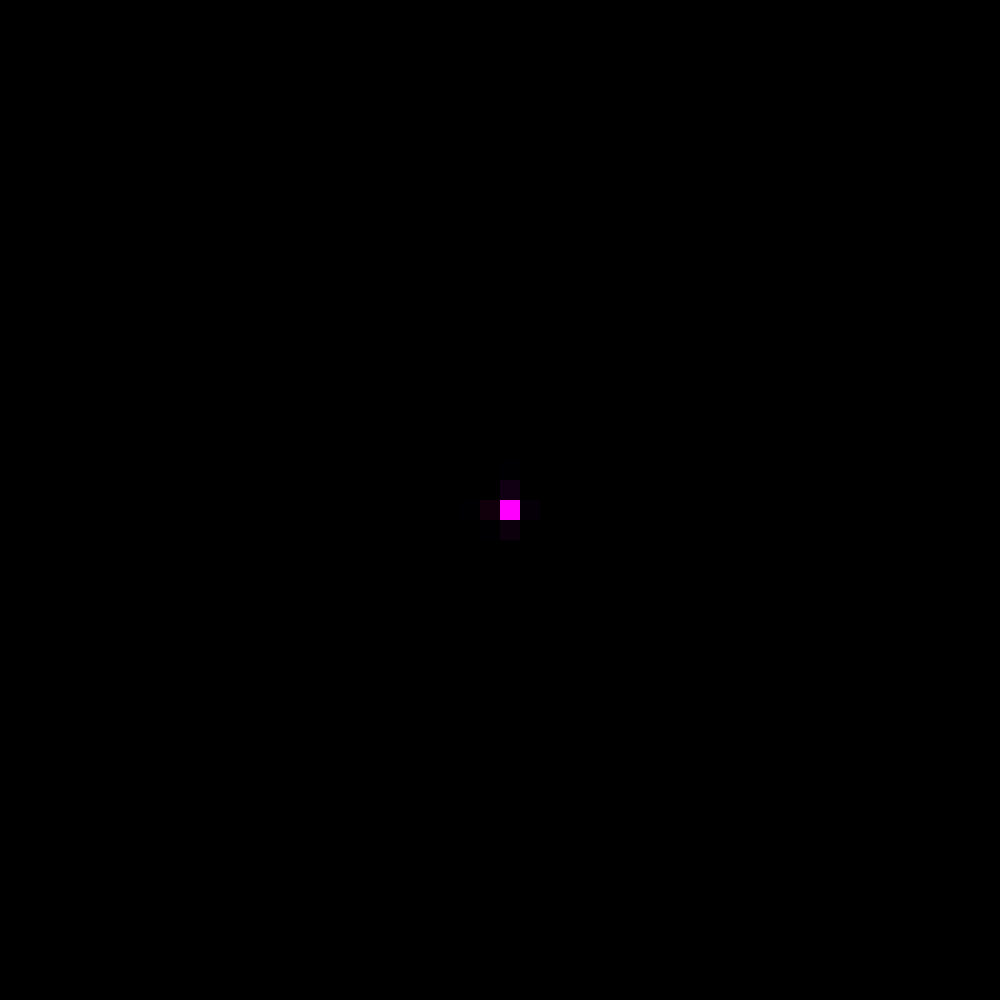
\includegraphics[height=0.8\textheight]{dsrd2d}}{dsrd2d.mp4}
\movie{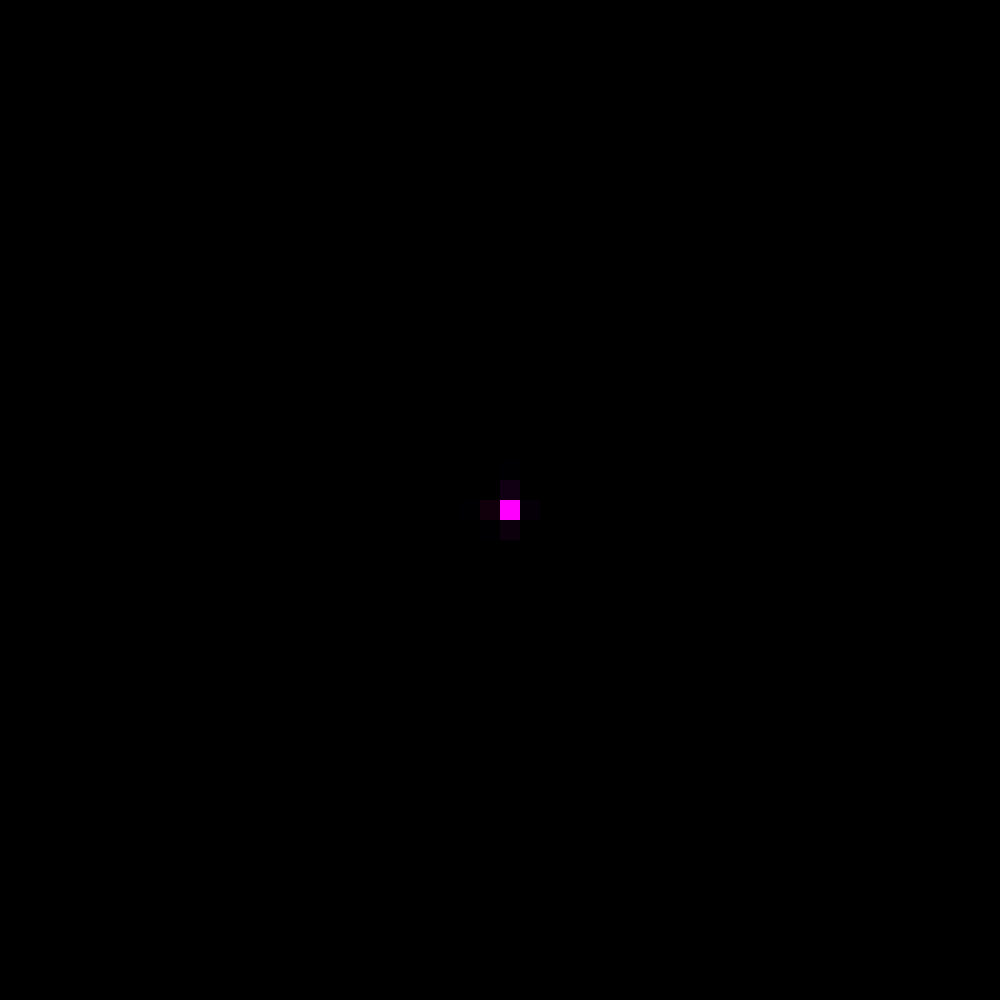
\includegraphics[height=0.85\textheight]{dsrd2d}}{dsrd2d.mp4}
\end{center}
}

\begin{comment}

  \frame{
\frametitle{Spatial CLE approximation}
\begin{center}
%\movie[externalviewer]{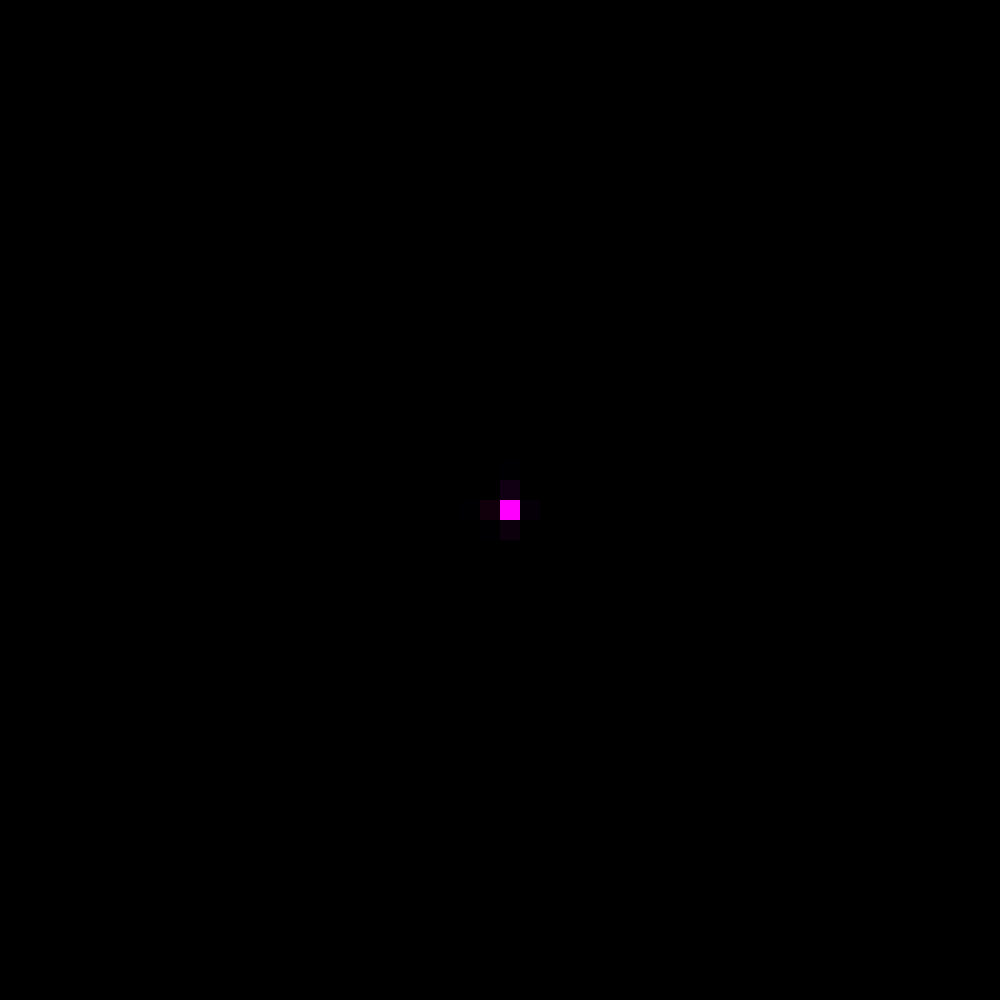
\includegraphics[height=0.8\textheight]{dsrd2d}}{sgrd2d.mp4}
\movie{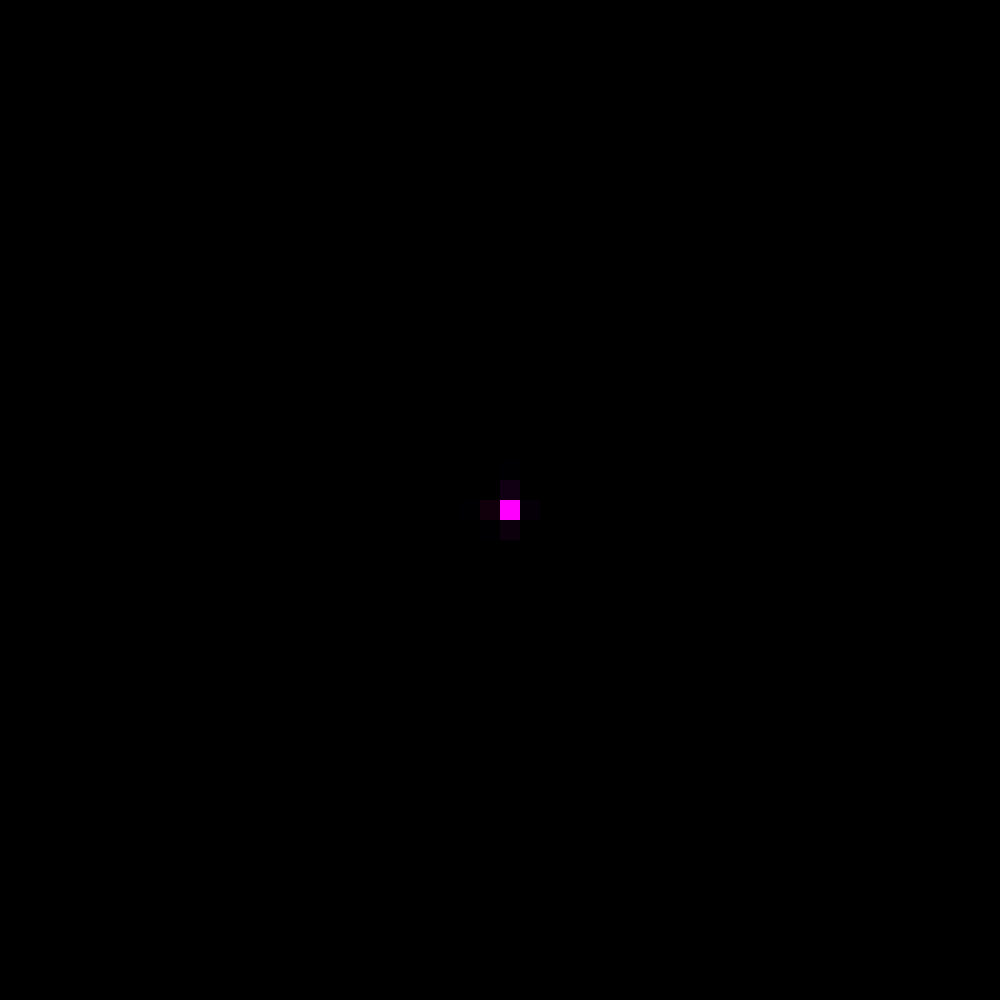
\includegraphics[height=0.85\textheight]{dsrd2d}}{sgrd2d.mp4}
\end{center}
}


\frame{
\frametitle{SDE approximation on a fine grid}
\begin{center}
%\movie[externalviewer]{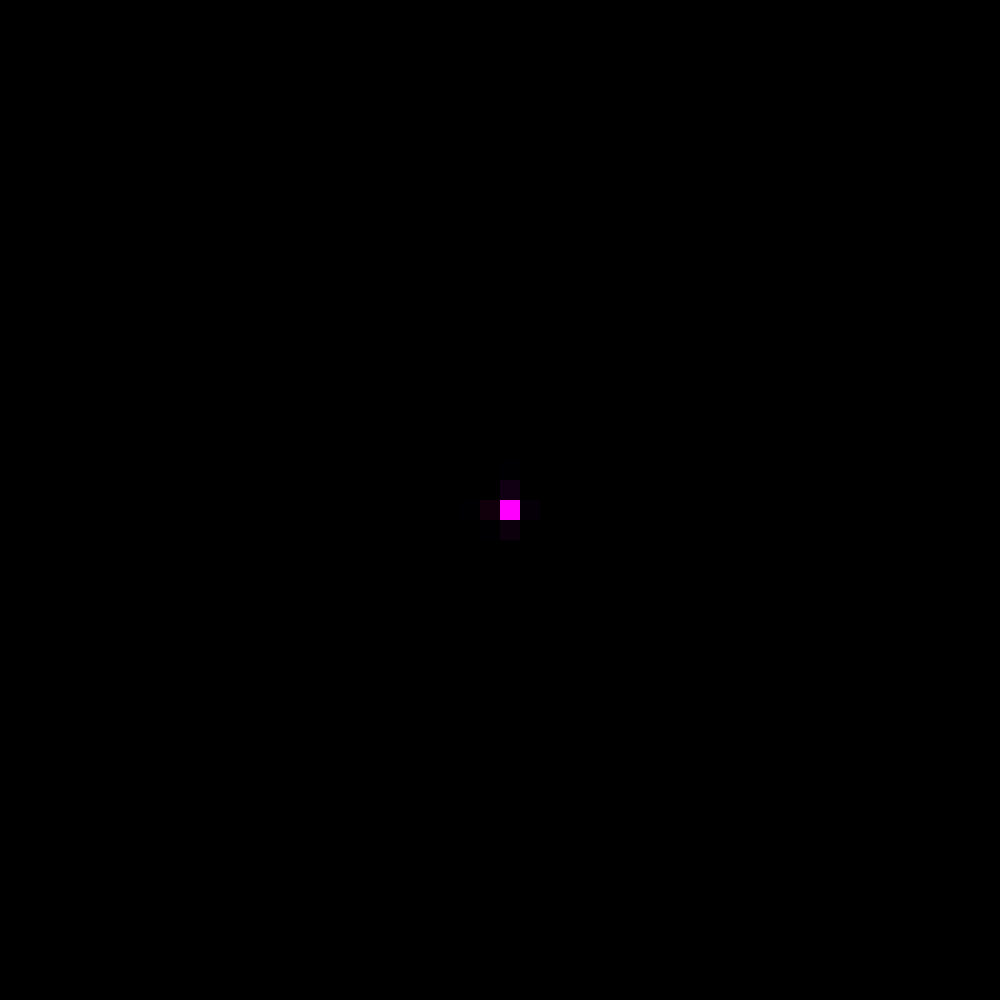
\includegraphics[height=0.8\textheight]{dsrd2d}}{sgrd2dv2.mp4}
\movie{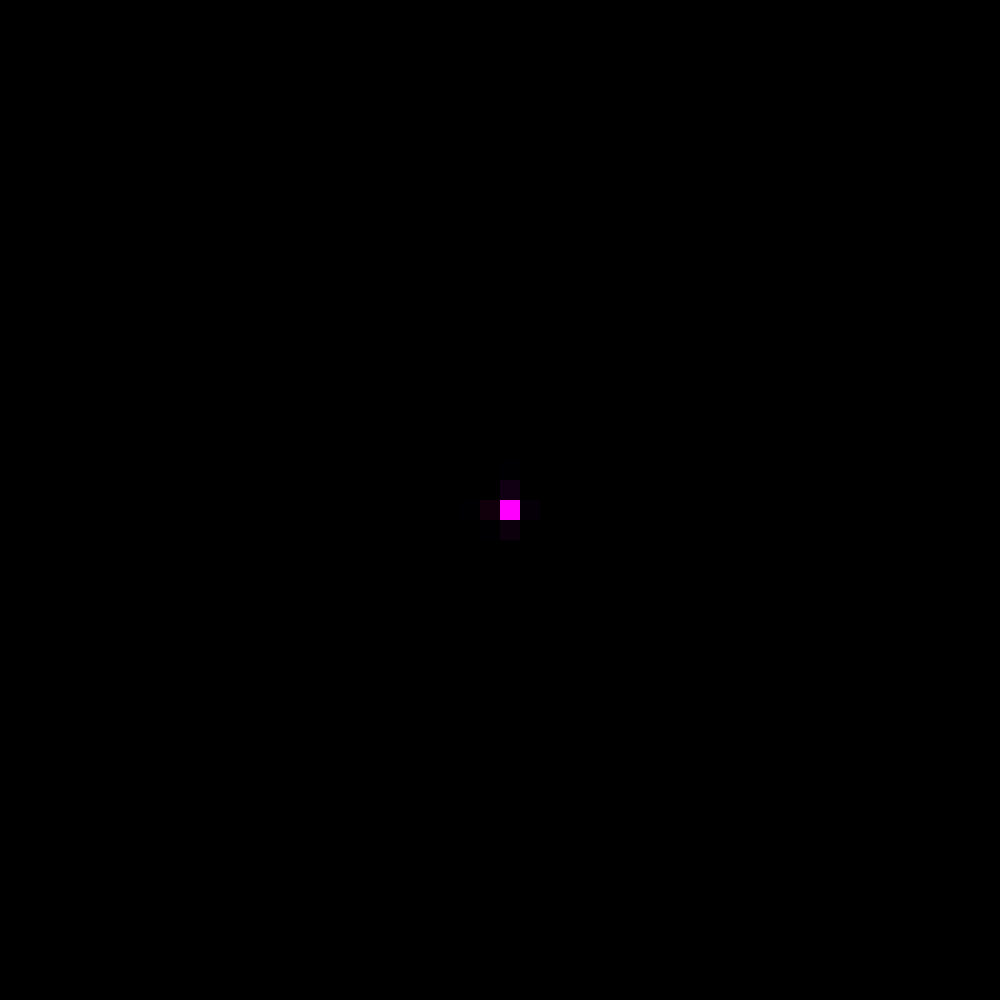
\includegraphics[height=0.8\textheight]{dsrd2d}}{sgrd2dv2.mp4}
\end{center}
}

\end{comment}

\frame{
\frametitle{Lotka--Volterra SPDE dynamics (via the spatial CLE)}
\begin{center}
%\movie[externalviewer]{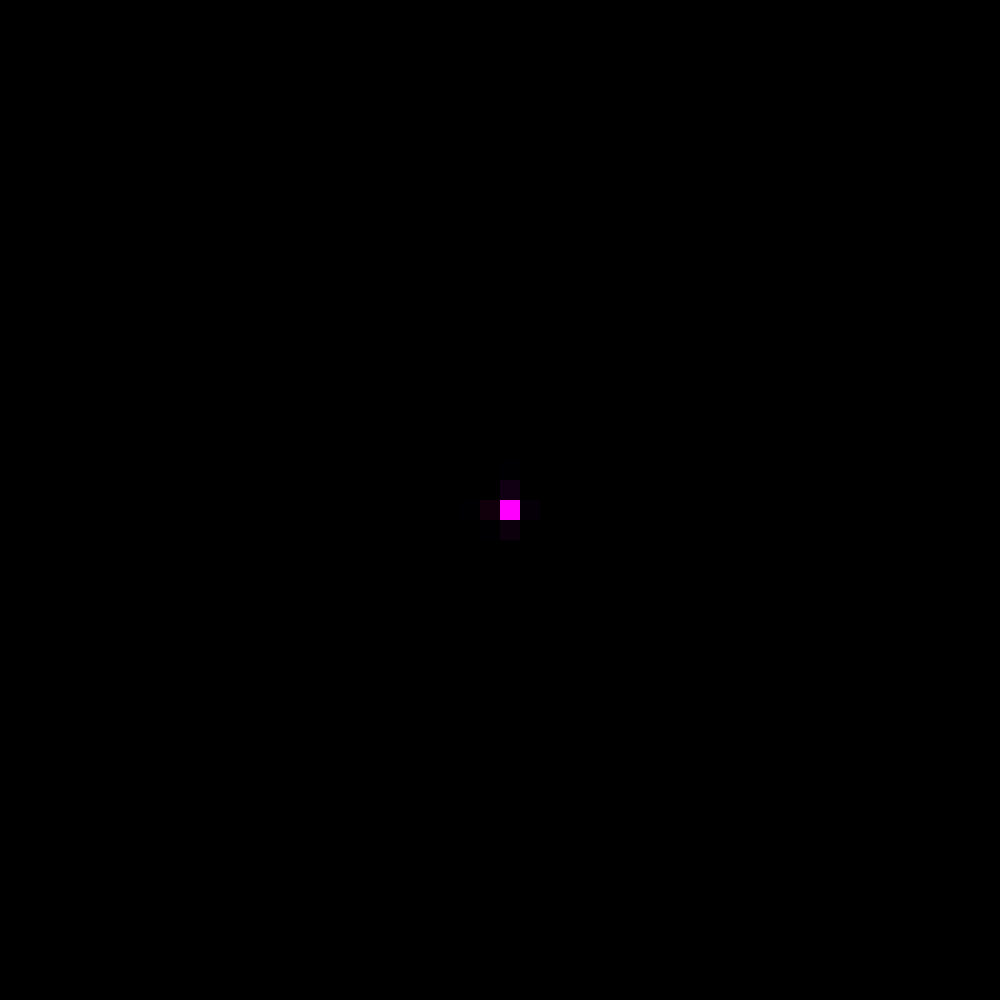
\includegraphics[height=0.8\textheight]{dsrd2d}}{sgrd2dv3.mp4}
\movie{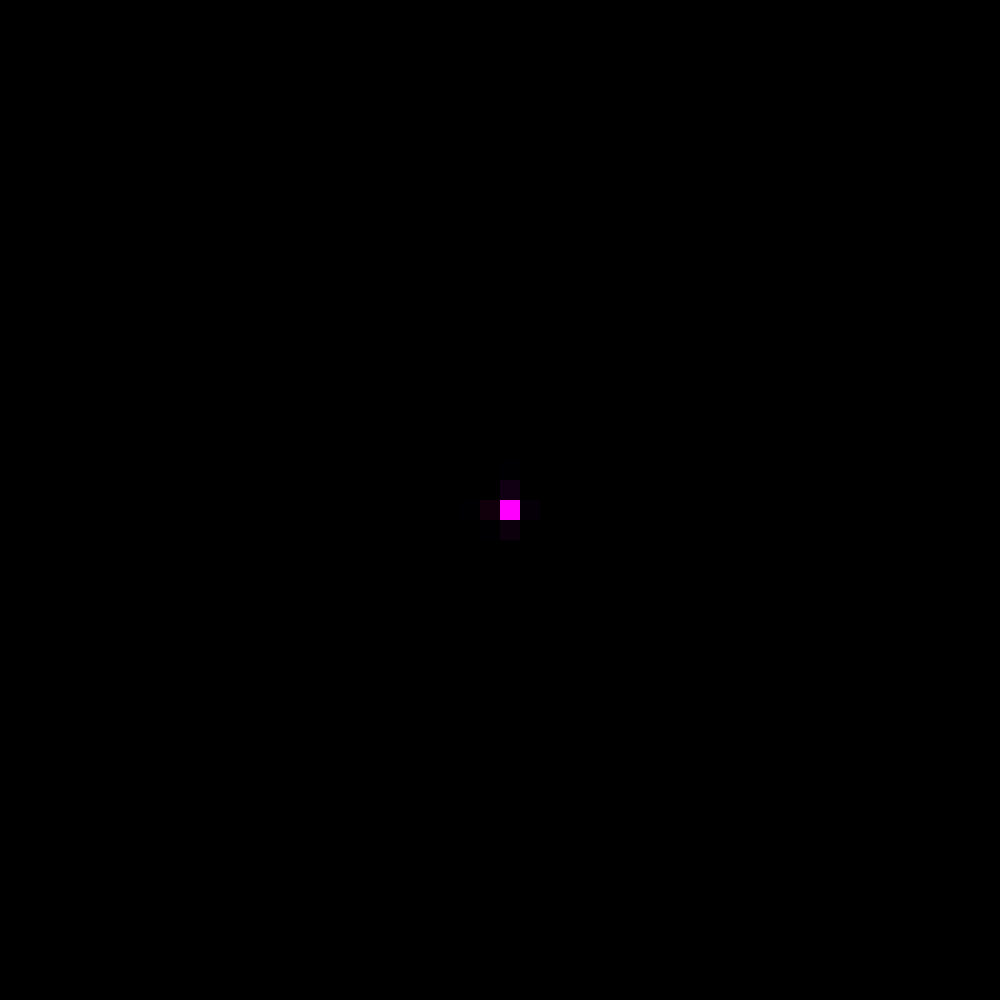
\includegraphics[height=0.85\textheight]{dsrd2d}}{sgrd2dv3.mp4}
\end{center}
}

\begin{comment}

\frame{
\frametitle{Lotka--Volterra SPDE dynamics (3 seeds)}
\begin{center}
%\includemovie{.8\textheight}{.8\textheight}{sgrd2dv4.mp4}
%\movie[externalviewer]{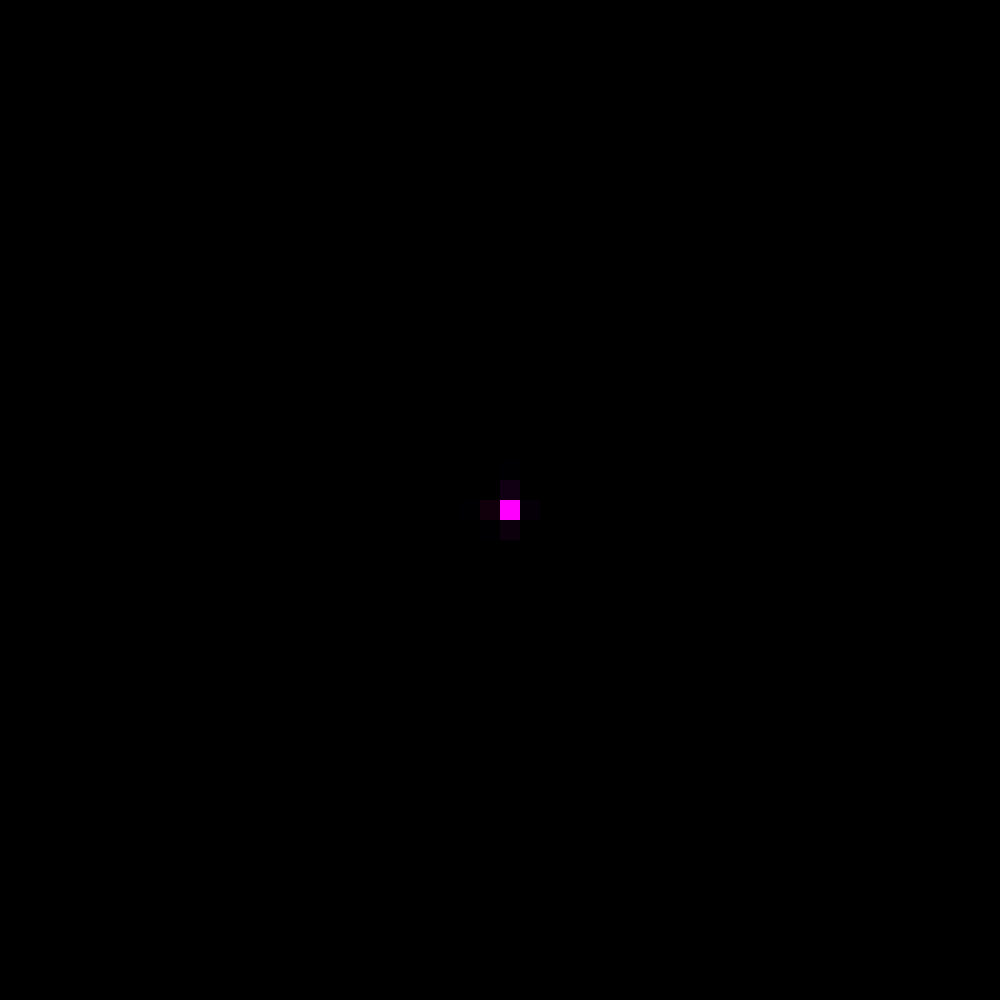
\includegraphics[height=0.8\textheight]{dsrd2d}}{sgrd2dv4.mp4}
\movie{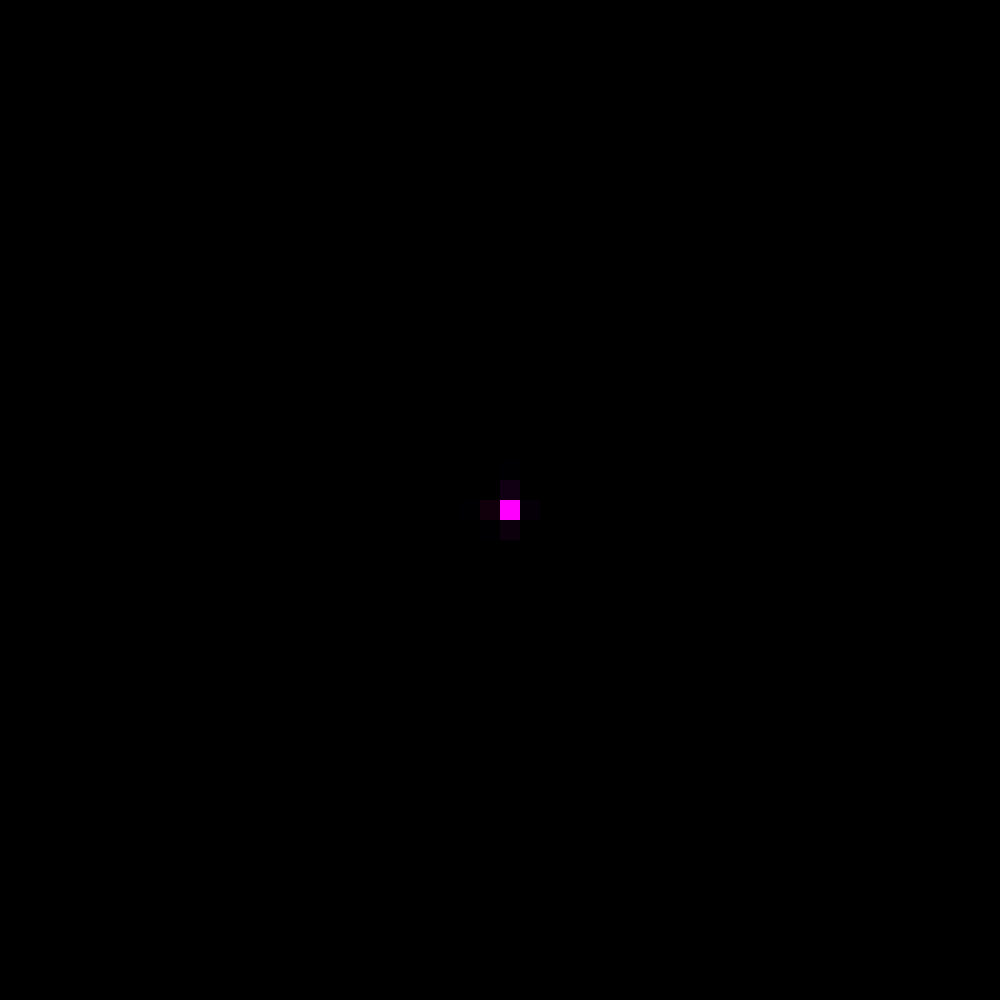
\includegraphics[height=0.85\textheight]{dsrd2d}}{sgrd2dv4.mp4}
\end{center}
}

\end{comment}

\frame{
  \frametitle{Lotka--Volterra reaction--diffusion SPDE}
    \vspace*{-5cm}\centerline{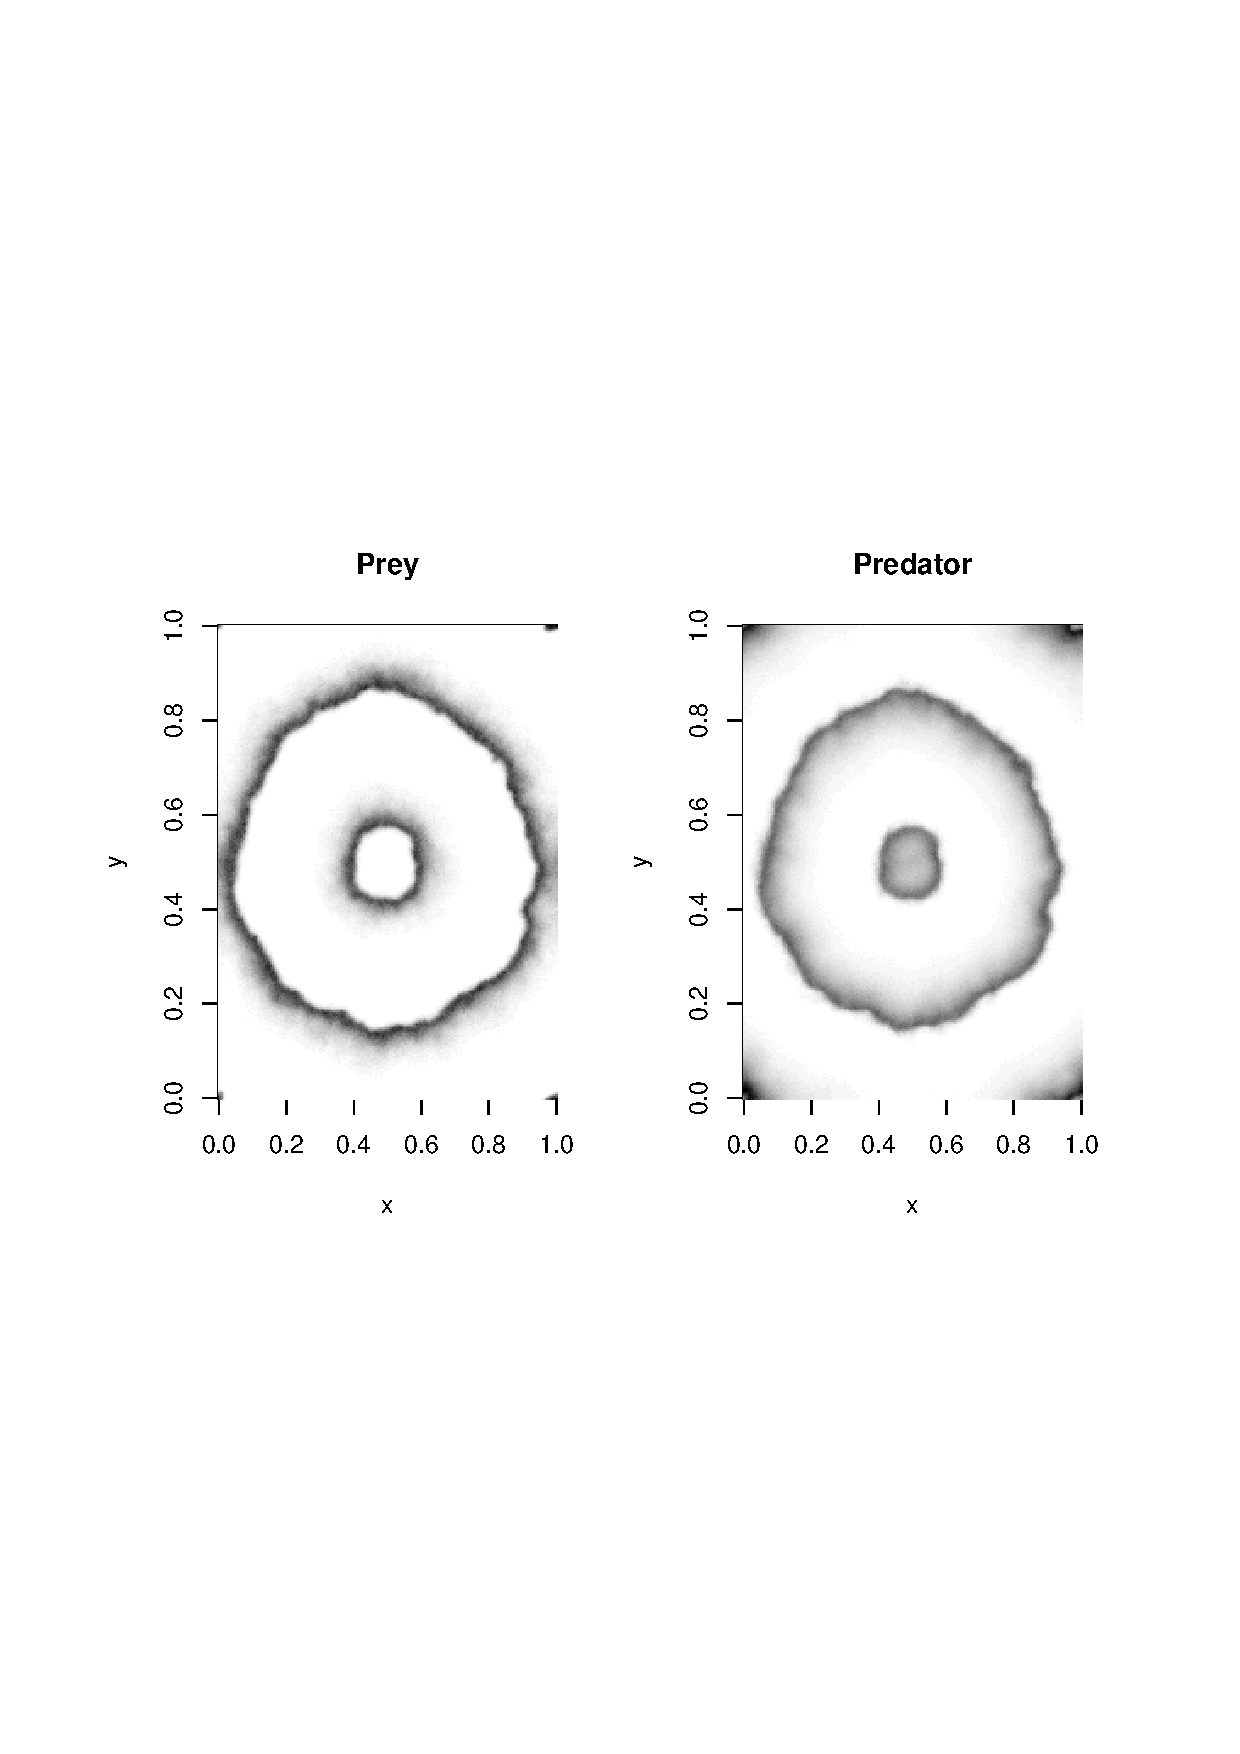
\includegraphics[width=1.2\textwidth]{figs/ch09scle2dex2}}
}


\frame{
  \frametitle{Modularity and simulation algorithms}
  \begin{itemize}
  \item Separating models from simulation algorithms has many benefits
  \item Separating model parameters from models so that simulation algorithms don't need to know about parameters is similarly beneficial
  \item Models can be simulated in different ways, using different algorithms, and under different assumptions: exact/approximate, discrete/continuous, stochastic/deterministic, well-mixed/spatial, ...
    \item Model exchange formats, such as SBML, can be useful for understanding some of the issues
    \end{itemize}
  }

%\section{Bayesian inference}

%\subsection{Overview}

\frame{
\frametitle{Parameter inference}
\begin{itemize}
\item The auto-regulatory network model contains 5 species and 8 reactions
\item Each reaction has an associated \alert{rate constant} --- these 8 rate constants may be subject to uncertainty
\item The \alert{initial state} of the model (5 species levels) may also be uncertain/unknown
\item There could also be uncertainty about the \alert{structure of the reaction network} itself --- eg. presence/absence of particular reactions --- this can be embedded into the parameter inference problem, but is often considered separately, and is not the subject of this talk
\item We will focus here on using \alert{time course data} on some aspect of one (or more) realisations of the underlying stochastic process in order to make inferences for any unknown parameters of the model
\end{itemize}
}

\frame{
\frametitle{Partial, noisy data on the auto-reg model}
\centerline{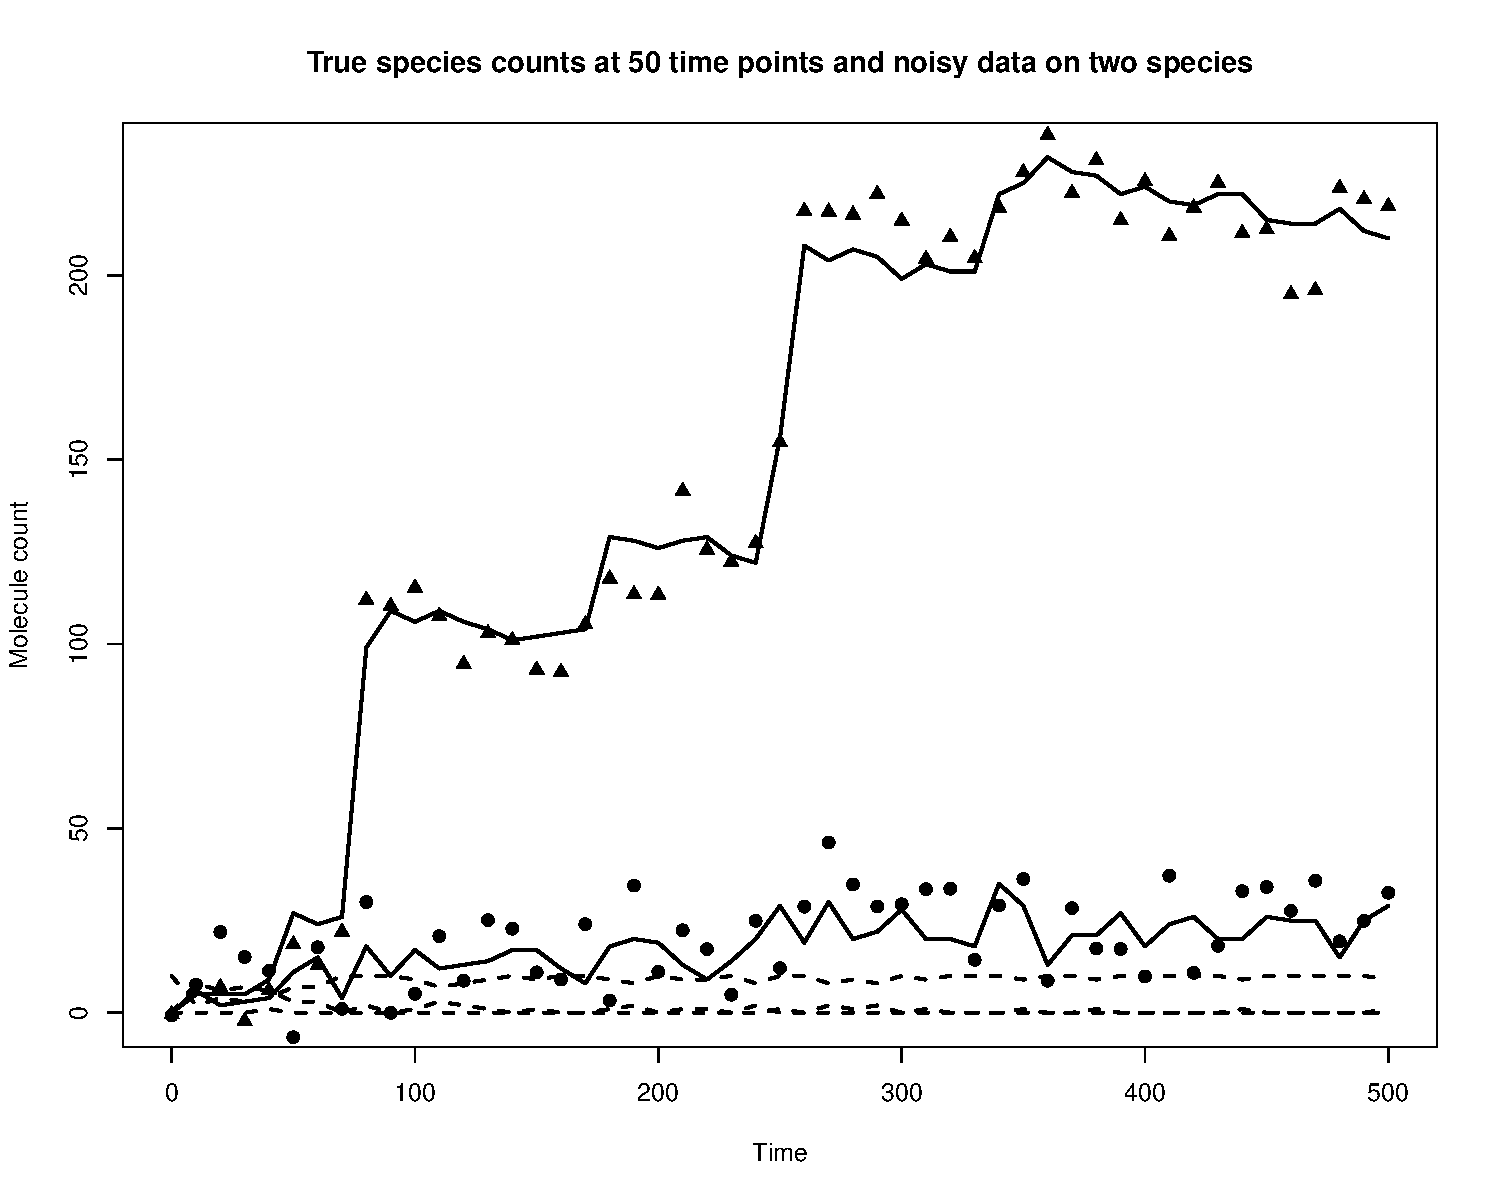
\includegraphics[height=0.9\textheight]{figs/ar/AR-Data}}
}



\frame{
\frametitle{Classes of Bayesian Monte Carlo algorithms}
In this context there are 3 main classes of MC algorithms:
\begin{itemize}
\item \alert{ABC algorithms} (likelihood--free)
 \begin{itemize}
 \item Completely general (in principle) ``global'' Approximate Bayesian Computation algorithms, so just require a forward simulator, and don't rely on (eg.) Markov property, but typically very inefficient and approximate
 \end{itemize}
\item \alert{POMP algorithms} (likelihood--free)
 \begin{itemize}
 \item Typically ``local'' (particle) MCMC-based algorithms for Partially Observed Markov Processes, again only requiring a forward simulator, but using the Markov property of the process for improved computational efficiency and ``exactness''
 \end{itemize}
\item \alert{Likelihood-based MCMC algorithms}
 \begin{itemize}
 \item More efficient (exact) MCMC algorithms for POMP models, working directly with the model representation, not using a forward simulator, and requiring the evaluation of likelihoods associated with the \alert{sample paths} of the stochastic process
 \end{itemize}
\end{itemize}
}

\frame{
\frametitle{Modularity and model decoupling for inference}
\small
\begin{itemize}
\item Decoupling the model from the inference algorithm is just as important as separation of the model from a forward simulation algorithm
\item The key characteristic of \alert{likelihood-free} (or ``plug-and-play'') algorithms is that they separate inference algorithms from the forward simulator completely --- this strong decoupling has many advantages, with the main disadvantage being the relative inefficiency of the inferential algorithms
\item The likelihood-free algorithms rely heavily on forward simulation, so can immediately benefit from improvements in exact and approximate simulation technology
\item There is no reason why efficient likelihood-based MCMC algorithms can't also be decoupled from the model representation, but doing so for a reasonably large and flexible class of models seems to be beyond the programming skills of most statisticians...
\end{itemize}
}

%\subsection{POMP Models}

\frame{
\frametitle{Partially observed Markov process (POMP) models}
\begin{itemize}
\item Continuous-time Markov process: $\mathbf{X}=\{X_s|s\geq 0\}$ (for now, we
  suppress dependence on parameters, $\theta$)
\item Think about integer time observations (extension to arbitrary
  times is trivial): for $t\in \mathbb{N},\quad
  \mathbf{X}_t=\{X_s|t-1<s\leq t\} $
\item Sample-path likelihoods such as $\pi(\mathbf{x}_t|x_{t-1})$ can
  often (but not always) be computed (but are often computationally
  difficult), but discrete time transitions such as $\pi(x_t|x_{t-1})$
  are typically intractable
\item Partial observations: $\mathcal{Y}=\{y_t|t=1,2,\ldots,T\}$ where
\[
y_t|X_t=x_t \sim \pi(y_t|x_t), \qquad t=1,\ldots,T,
\]
where we assume that $\pi(y_t|x_t)$ can be evaluated directly (simple
measurement error model)
\end{itemize}
}

\frame{
\frametitle{Bayesian inference for latent process models}
\begin{itemize}
\item Vector of \alert{model parameters}, $\theta$, the object of inference
\item Prior probability distribution on $\theta$, denoted $\pi(\theta)$
\item Conditional on $\theta$, we can simulate realisation of the \alert{stochastic process} $\mathbf{X}$, with probability model $\pi(\mathbf{x}|\theta)$, which may be intractable
\item \alert{Observational data} $\mathcal{Y}$, determined from $\mathbf{x}$ and $\theta$ by a the probability model $\pi(\mathcal{Y}|\mathbf{x},\theta)$ --- for ``exact'' algorithms we typically require that this model is tractable, but for ABC, we only need to be able to simulate from it
\item Joint model $\pi(\theta,\mathbf{x},\mathcal{Y}) = \pi(\theta)\pi(\mathbf{x}|\theta)\pi(\mathcal{Y}|\mathbf{x},\theta)$
\item \alert{Posterior distribution} $\pi(\theta,\mathbf{x}|\mathcal{Y}) \propto \pi(\theta,\mathbf{x},\mathcal{Y})$
\item If using Monte Carlo methods, easy to marginalise out $\mathbf{x}$ from samples from the posterior to get samples from the parameter posterior $\pi(\theta|\mathcal{Y})$
\end{itemize}
}


\frame{
\frametitle{Likelihood-free PMMH pMCMC}
\begin{itemize}
\item \alert{Particle Markov chain Monte Carlo} (pMCMC) methods are a powerful tool for parameter inference in POMP models
\item In the variant known as \alert{particle marginal Metropolis Hastings} (PMMH), a (random walk) MH MCMC algorithm is used to explore parameter space, but at each iteration, a (bootstrap) particle filter (SMC algorithm) is run to calculate terms required in the acceptance probability
\item The ``magic'' of pMCMC is that despite the fact that the particle filters are ``approximate'', pMCMC algorithms nevertheless have the ``exact'' posterior distribution of interest (either  $\pi(\theta|\mathcal{Y})$ or $\pi(\theta,\mathbf{x}|\mathcal{Y})$) as their target
\item If a sophisticated particle filter is used, pMCMC can be a reasonably efficient likelihood-based MCMC method --- however, when a simple ``bootstrap'' particle filter is used, the entire process is ``likelihood-free'', but still ``exact''
\end{itemize}
}

\begin{comment}

\frame{
\frametitle{Particle MCMC (pMCMC)}
\begin{itemize}
\item pMCMC is the only obvious practical
  option for constructing a global likelihood-free MCMC algorithm for POMP models which
  is exact (\alert{\href{http://dx.doi.org/10.1111/j.1467-9868.2009.00736.x}{Andrieu et al, 2010}})
\item Start by considering a basic marginal MH MCMC scheme with target
  $\pi(\theta|\mathcal{Y})$ and proposal $f(\theta^\star|\theta)$ ---
  the acceptance probability is $\min\{1,A\}$ where
\[
A = \frac{\pi(\theta^\star)}{\pi(\theta)}\times
\frac{f(\theta|\theta^\star)}{f(\theta^\star|\theta)}\times \frac{\pi(\mathcal{Y}|\theta^\star)}{\pi(\mathcal{Y}|\theta)}
\]
\item We can't evaluate the final terms, but if we had a way to
  construct a Monte Carlo estimate of the likelihood,
  $\hat\pi(\mathcal{Y}|\theta)$, we could just plug this in and hope
  for the best:
\[
A = \frac{\pi(\theta^\star)}{\pi(\theta)}\times
\frac{f(\theta|\theta^\star)}{f(\theta^\star|\theta)}\times \frac{\hat\pi(\mathcal{Y}|\theta^\star)}{\hat\pi(\mathcal{Y}|\theta)}
\]
\end{itemize}
}


\frame{
\frametitle{``Exact approximate'' MCMC (the pseudo-marginal approach)}
\begin{itemize}
\item
Remarkably, provided only that
$\operatorname{E}[\hat\pi(\mathcal{Y}|\theta)]=\pi(\mathcal{Y}|\theta)$,
the stationary distribution of the Markov chain will be
\alert{exactly} correct (\alert{\href{http://www.genetics.org/cgi/content/abstract/164/3/1139}{Beaumont, 2003}}, \alert{\href{http://dx.doi.org/10.1214/07-AOS574}{Andrieu \& Roberts, 2009}})
\item
Putting $W=\hat\pi(\mathcal{Y}|\theta)/\pi(\mathcal{Y}|\theta)$ and
augmenting the state space of the chain to include $W$, we find that
the target of the chain must be
\[
\propto \pi(\theta)\hat\pi(\mathcal{Y}|\theta)\pi(w|\theta) \propto
\pi(\theta|\mathcal{Y})w\pi(w|\theta)
\]
and so then the above ``unbiasedness'' property implies that
$\operatorname{E}(W|\theta)=1$, which
guarantees that the marginal for $\theta$ is exactly
$\pi(\theta|\mathcal{Y})$
%\item Blog post: \alert{\url{http://tinyurl.com/6ex4xqw}}
\end{itemize} 
}



\frame{
\frametitle{Particle marginal Metropolis-Hastings (PMMH)}
\begin{itemize}
\item Likelihood estimates constructed via importance sampling typically have
  this ``unbiasedness'' property, as do estimates constructed using a
  particle filter
\item If a particle filter is used to construct the Monte Carlo
  estimate of likelihood to plug in to the acceptance probability, we
  get (a simple version of) the particle Marginal Metropolis Hastings
  (PMMH) pMCMC algorithm
\item The full PMMH algorithm also uses the particle filter to
  construct a proposal for $\mathbf{x}$, and has target
  $\pi(\theta,\mathbf{x}|\mathcal{Y})$ --- not just
  $\pi(\theta|\mathcal{Y})$
\item The (bootstrap) particle filter relies only on the ability to
  forward simulate from the process, and hence the entire procedure is
  ``likelihood-free''
\end{itemize} 
% Blog post: \alert{\url{http://bit.ly/kvznmq}}
See \alert{Golightly and W (2011)} for further details
}


\end{comment}

\frame{
\frametitle{PMMH inference results}
\centerline{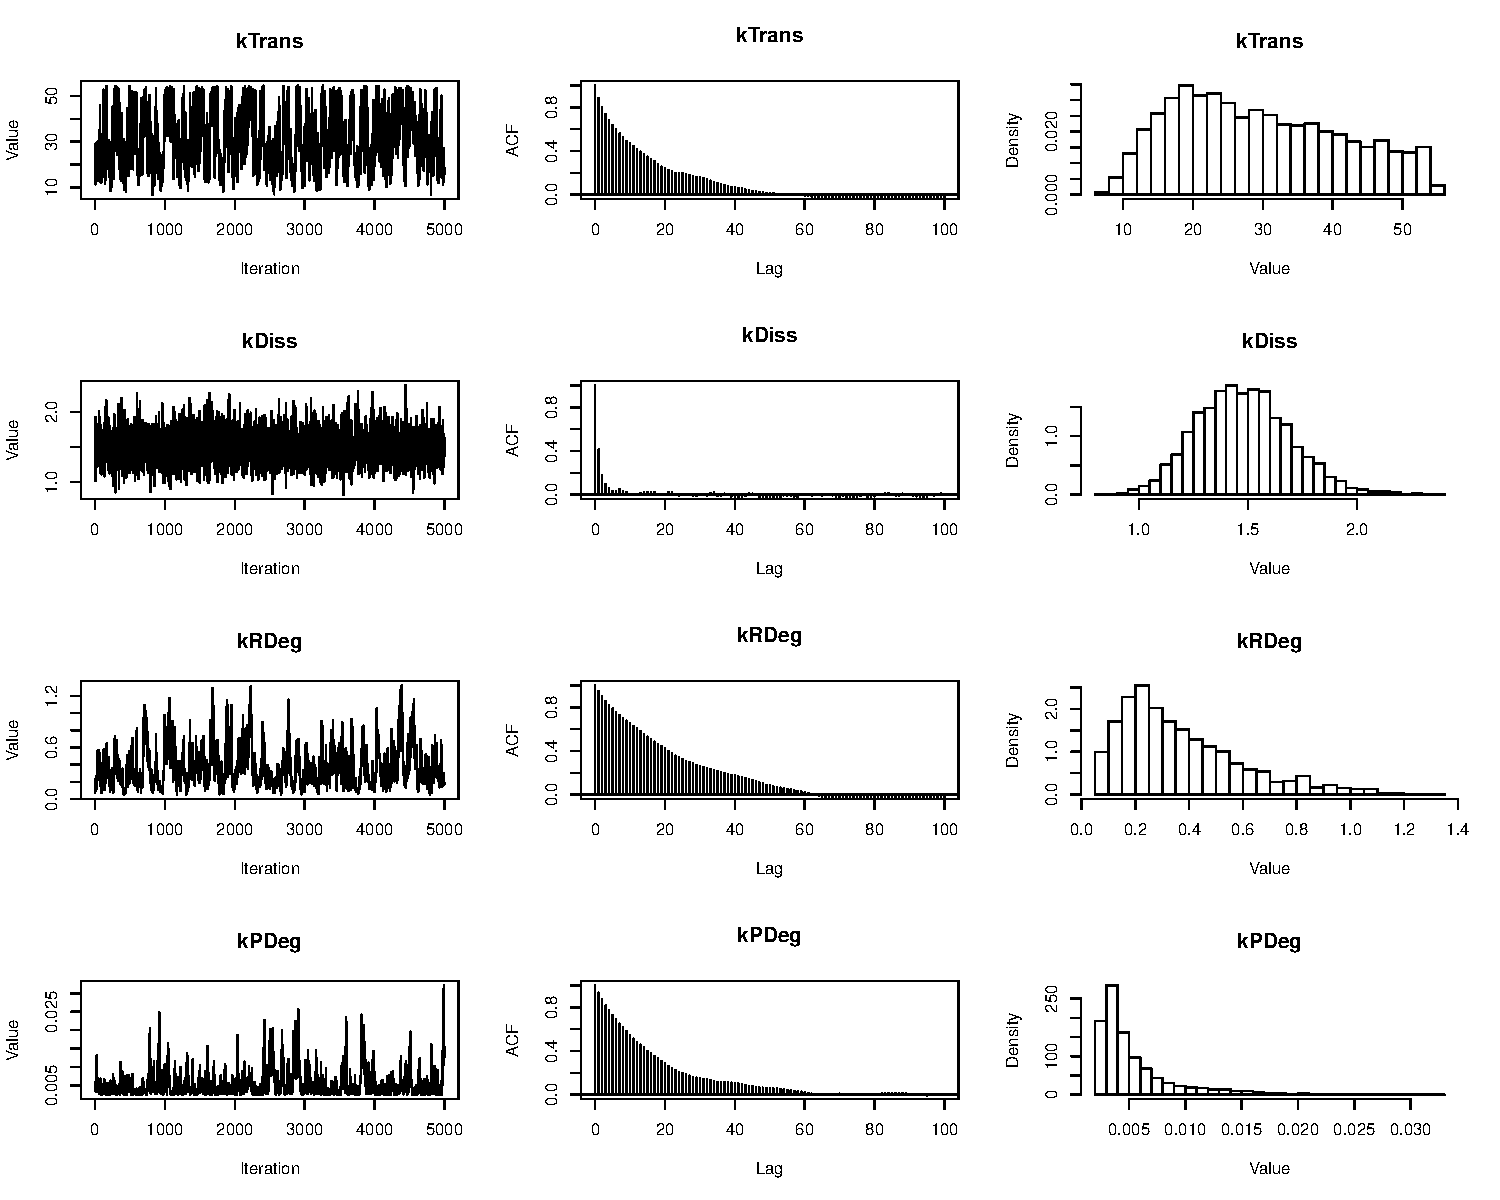
\includegraphics[height=0.9\textheight]{figs/ar/AR-Pmmh100k-240-t-tr}}
}

\begin{comment}
  
\frame{
\frametitle{PMMH inference results}
\centerline{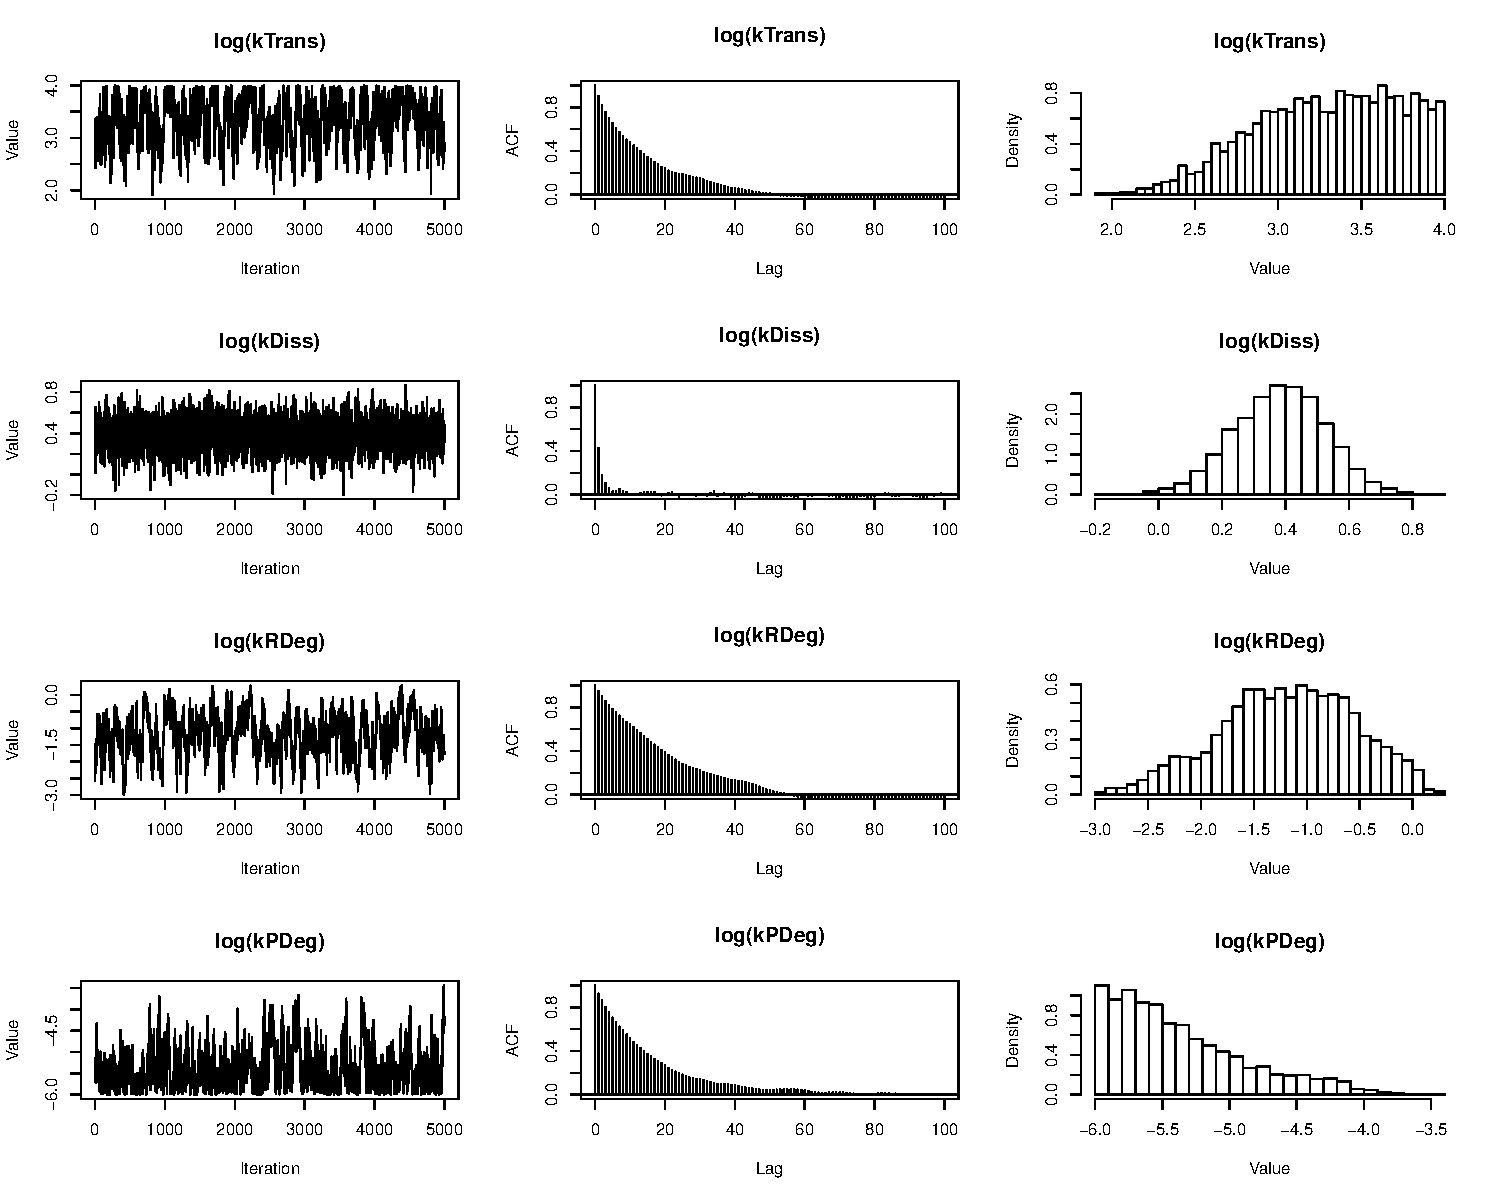
\includegraphics[height=0.9\textheight]{figs/ar/AR-Pmmh100k-240-t-log-tr}}
}

\frame{
\frametitle{PMMH inference results}
\centerline{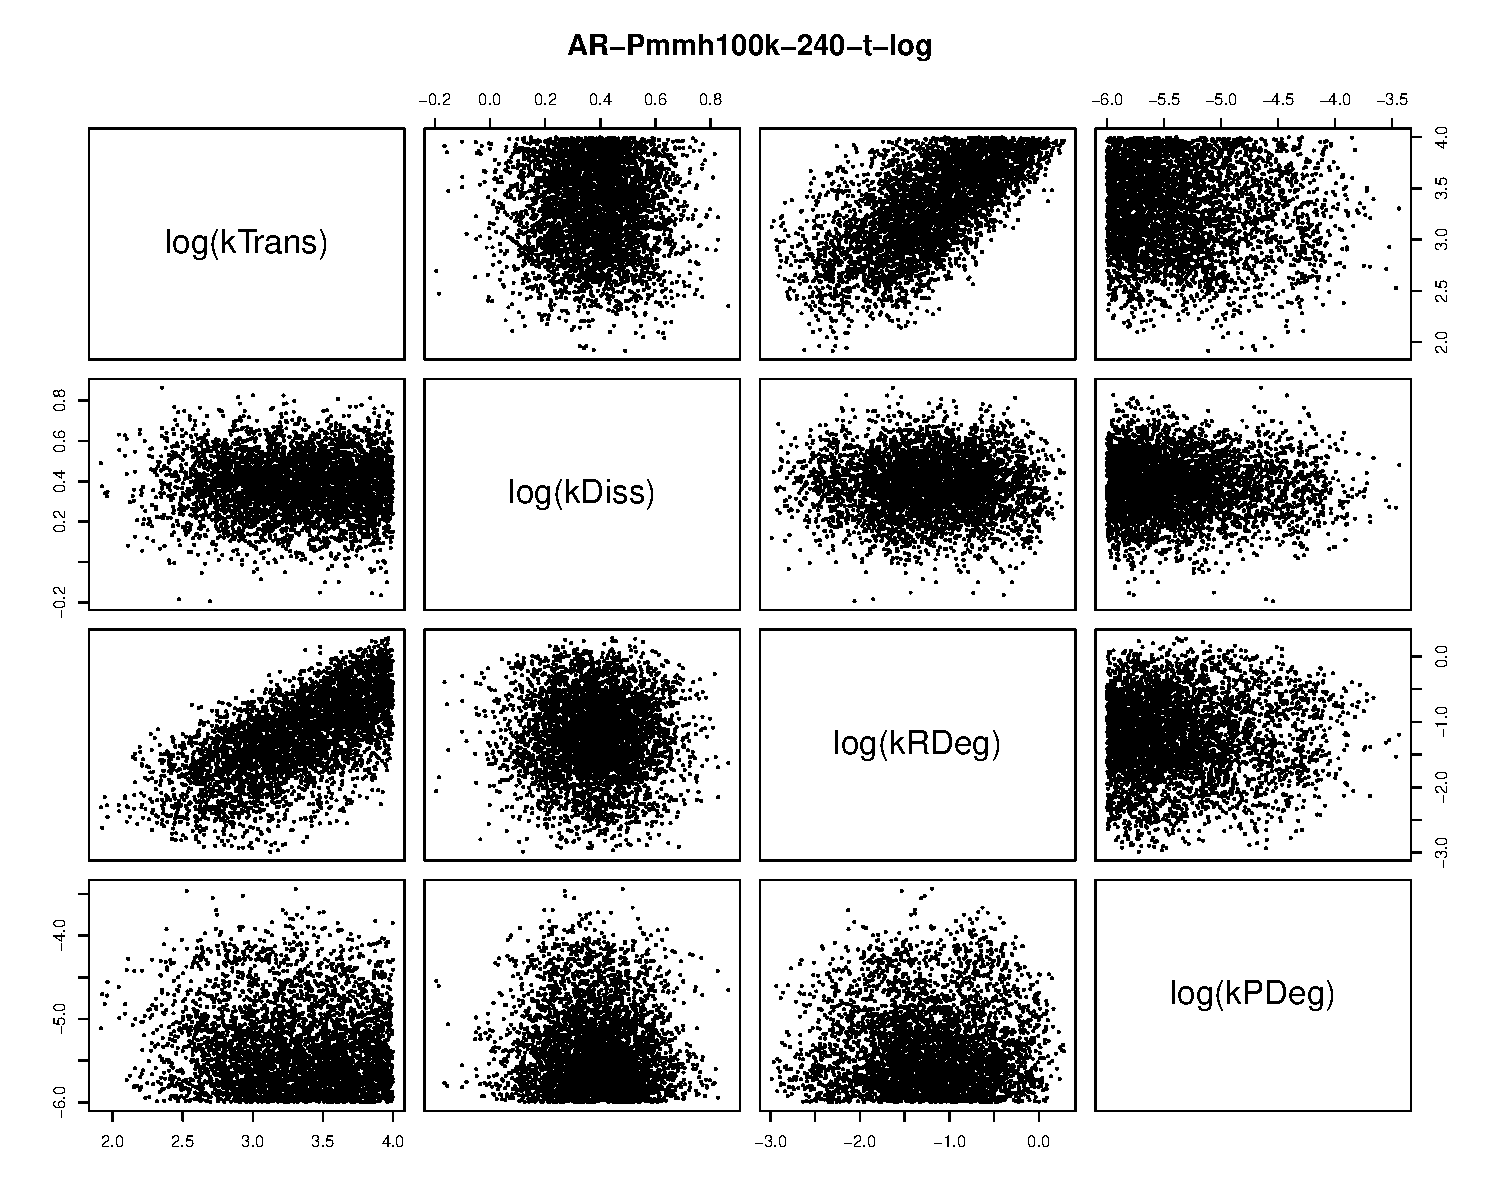
\includegraphics[height=0.9\textheight]{figs/ar/AR-Pmmh100k-240-t-log-sc}}
}

\end{comment}

\frame{
\frametitle{``Sticking'' and tuning of PMMH}
\begin{itemize}
\item As well as tuning the $\theta$ proposal variance, it is
  necessary to tune the number of particles, $N$ in the particle filter ---
  need enough to prevent the chain from sticking, but computational
  cost roughly linear in $N$
\item
Number of particles necessary depends on $\theta$, but don't know
$\theta$ \emph{a priori}
\item Initialising the sampler is non-trivial, since much of parameter
  space is likely to lead to likelihood estimates which are dominated by noise --- how to move around when you don't know which way is ``up''?!
\item Without careful tuning and initialisation, burn-in, convergence
  and mixing can all be very problematic, making algorithms painfully slow...
\end{itemize}
}


\begin{comment}
  
\frame{
\frametitle{General SIR particle filter}
\begin{itemize}
\item At time $t$, we have (after resampling) an equally weighted sample from $\pi(x_t|y_{1:t})$
\item At time $t+1$, we want a weighted sample from $\pi(x_{t+1}|y_{1:t+1})$, though in fact useful to construct a sample from $\pi(x_{t+1},x_t|y_{1:t+1})$, and then marginalise down as required
\item Target $\propto \pi(y_{t+1}|x_{t+1})\pi(x_{t+1}|x_t)\pi(x_t|y_{1:t})$ and proposal is $f(x_{t+1}|x_t,y_{t+1})\pi(x_t|y_{1:t})$, for some $f(\cdot)$, leading to unnormalised weight
\[
w_{t+1}= \frac{\pi(y_{t+1}|x_{t+1})\pi(x_{t+1}|x_t)}{f(x_{t+1}|x_t,y_{t+1})}
\]
\item LF choice is $f(x_{t+1}|x_t,y_{t+1})=\pi(x_{t+1}|x_t)$, otherwise need to evaluate the discrete time transition density
\end{itemize}
}

\frame{
\frametitle{Weights and RN derivatives}
\begin{itemize}
\item For Markov processes with intractable kernels, make the target $\pi(\mathbf{x}_{t+1},x_t|y_{1:t+1})$ and then marginalise down to $\pi(x_{t+1}|y_{1:t+1})$ if required
\item The proposal path will be of the form $f(\mathbf{x}_{t+1}|x_t,y_{t+1})\pi(x_t|y_{1:t})$, leading to weight
\[
w_{t+1} = \pi(y_{t+1}|x_{t+1})\frac{\pi(\mathbf{x}_{t+1}|x_t)}{f(\mathbf{x}_{t+1}|x_t,y_{t+1})}
\]
\item The expected weight is $\pi(y_{t+1}|y_{1:t})$, as needed for pseudo-marginal MCMC
\item Formally,
\[
w_{t+1}= \pi(y_{t+1}|x_{t+1})\frac{d\mathbb{P}}{d\mathbb{Q}}(\mathbf{x}_{t+1}|x_t),
\]
the RN derivative of the true (unconditioned) diffusion wrt the proposal process
\end{itemize}
}

\end{comment}

%\subsection{ABC approaches}


%%\subsection{ABC}


\frame{
\frametitle{Alternative: approximate Bayesian computation (ABC)}
\begin{itemize}
\item Since
  $\pi(\theta,\mathbf{x},\mathcal{Y})=\pi(\theta)\pi(\mathbf{x}|\theta)\pi(\mathcal{Y}|\theta,\mathbf{x})$, it is trivial to generate samples from $\pi(\theta,\mathbf{x},\mathcal{Y})$ and to marginalise these down to $\pi(\theta,\mathcal{Y})$ 
\item Exact rejection algorithm: generate
  $(\theta^\star,\mathcal{Y}^\star)$ from $\pi(\theta,\mathcal{Y})$
  and keep provided that $\mathcal{Y}=\mathcal{Y}^\star$ otherwise
  reject and try again
\item This gives exact realisations from $\pi(\theta|\mathcal{Y})$,
  but in practice the acceptance rate will be very small (or zero)
\item ABC: Define a metric on the sample space, $\rho(\cdot,\cdot)$,
  and accept $(\theta^\star,\mathcal{Y}^\star)$ if
  $\rho(\mathcal{Y},\mathcal{Y}^\star)<\eps$
\item  This gives exact realisations from
  $\pi(\theta|\rho(\mathcal{Y},\mathcal{Y}^\star)<\eps)$, which tends
  to the true posterior as $\eps\longrightarrow 0$
\item Still problematic if there is a large discrepancy between the
  prior and posterior...
\end{itemize}
}


\frame{
\frametitle{Summary statistics}
\begin{itemize}
\item The choice of metric $\rho(\cdot,\cdot)$ is very important to the overall efficiency and performance of ABC methods
\item Using a naive Euclidean distance on the raw data $\rho(\mathcal{Y},\mathcal{Y}^\star)=\Vert\mathcal{Y}-\mathcal{Y}^\star\Vert$ is likely to perform poorly in practice --- even with a perfect choice of parameters, it is extremely unlikely that you will ``hit'' the data
\item Ideally, we would use a vector of \alert{sufficient statistics}, $s(\mathcal{Y})$ of the \alert{likelihood model} associated with the process, to summarise the important aspects of the data relevant to parameter inference, and then define a metric on $s(\cdot)$
\item In practice, for complex models we don't know the sufficient statistics (and they probably don't exist), but we nevertheless form a vector of \alert{summary statistics}, which we hope capture the important aspects of the process and ignore the irrelevant noise in each realisation
\end{itemize}
}

\begin{comment}

\frame{
\frametitle{Summary statistics for POMP models}
\begin{itemize}
\item For time series data, obvious summary statistics for each univariate component include the sample \alert{mean}, (log-)\alert{variance}, and the \alert{lag 1 and 2 auto-correlations}
\item For multivariate time series, the (matrix of) \alert{cross-correlation}(s) is also useful
\item Together these summary statistics capture much of the essential dynamic structure of multivariate time series
\item For our auto-reg network example, this reduces the dimension of the statistic we are trying to match from $50\times 2=100$ to $2\times 4+1=9$ --- not only a big reduction, but we are now trying to match statistics that are relatively robust to noise in the data 
\item The individual components of $s(\cdot)$ are on different scales, so need to re-weight (eg. by standardising) before applying a simple metric such as Euclidean distance
\end{itemize}
}

\end{comment}

\frame{
\frametitle{Issues with simple rejection ABC}
\begin{itemize}
\item There are \alert{two main problems} with naive rejection sampling based ABC:
 \begin{itemize}
 \item The first relates to the \alert{dimension of the data}, and this is (largely) dealt with by carefully choosing and weighting appropriate \alert{summary statistics}
 \item The second relates to the dimension of the parameter space...
 \end{itemize} 
\item If the \alert{dimension of the parameter space} is large, the posterior distribution is likely to have almost all of its mass concentrated in a tiny part of the space covered by the prior, so the chances of hitting on good parameters when sampling from the prior will be very small
\item Might be better to gradually ``zoom in'' on promising parts of the parameter space gradually over a series of iterations...
\end{itemize}
}

\frame{
\frametitle{ABC--SMC}
\begin{itemize}
\item Interest in a Bayesian posterior distribution
\[
\pi(\theta|x) \propto \pi(\theta)f(x|\theta)
\]
where $f(x|\theta)$ is intractable
\item Observed data $x_0$
\item Sequence of approximations
\[
\pi_t(\theta) = \pi(\theta|\rho(x,x_0)<\eps_t),
\]
where $\infty=\eps_0>\eps_1>\cdots>\eps_n>0$ and $\rho(\cdot,\cdot)$
is a suitable metric on data space
\item $\pi_0$ is the prior, and for sufficiently small $\eps_n$,
  hopefully $\pi_n$ not too far from the posterior, $\pi(\theta|x_0)$
\item Progressively reduce tolerances to improve agreement between
  successive distributions and hopefully improve acceptance rates
\end{itemize}
}

\begin{comment}

\frame{
\frametitle{ABC--SMC algorithm}
\begin{itemize}
\item Suppose we have a large (possibly weighted) sample of size $N$
  from $\pi_{t-1}(\theta)$, $\{\theta_1,\ldots,\theta_N\}$ with
  normalised weights $\tilde{w}_{t-1}^i$
\item Pick $\theta_i^\star \sim \pi_{t-1}(\theta)$ (weighted
  particles)
\item Perturb $\theta_i^{\star\star}\sim
  K(\theta_i^\star,\theta_i^{\star\star})$
\item Simulate $x^\star\sim f(x^\star|\theta^{\star\star})$ from
  intractable likelihood model
\item Accept only if $\rho(x^\star,x_0)<\eps_t$, otherwise reject go back to
  the start and pick another $\theta_i^\star$
\item Keep $\theta^{\star\star}$ as $i$th member of new sample, and
  compute its weight as
\[
w_t^i = \frac{\pi(\theta^{\star\star})}{\sum_{j=1}^N
  \tilde{w}_{t-1}^i K(\theta_j,\theta^{\star\star})}
\]
\item Once a sample of size $N$ is obtained, normalise weights and
  increment $t$
\end{itemize}
}

\frame{
\frametitle{ABC--SMC weight derivation}
\begin{itemize}
\item Why does the ABC-SMC algorithm work? In particular, where does
  the weight expression come from?
\item Need to view proposal on $\theta^{\star\star}$ and $x^\star$
  jointly, but with $\theta^\star$ integrated out
\[
\propto \int_\Theta \pi_{t-1}(\theta^\star)K(\theta^\star,\theta^{\star\star})f(x^\star|\theta^{\star\star})I[\rho(x_0,x^\star)<\eps_t]\,d\theta^\star
\]
\item Similarly, the target is
\[
\propto \pi(\theta^{\star\star})f(x^\star|\theta^{\star\star})I[\rho(x_0,x^\star)<\eps_t]
\]
\item Leads to weight
\[
w= \frac{\pi(\theta^{\star\star})}{\int_\Theta
  \pi_{t-1}(\theta^\star)K(\theta^\star,\theta^{\star\star})\,d\theta^\star}
\]
with obvious particle approximation, leading to the desired weight
\end{itemize}
}

\end{comment}




%%\section{Summary and conclusions}

%%\subsection{Summary}


\frame{
\frametitle{Pros and cons of ABC(--SMC)}
\begin{itemize}
\item All likelihood-free methods have a tendency to be very computationally intensive and somewhat inefficient
\item ABC is very general, and can be applied to arbitrary settings (eg. not just POMP models)
\item ABC methods parallelise very well, and hence can be useful for getting reasonably good approximations to be true posterior relatively quickly if suitable hardware is available
\item ABC is becoming increasingly popular outside of statistics, where the idea of ``moment matching'' is familiar and intuitive
\item ABC usually results in a distribution significantly over-dispersed relative to the true posterior
\item The tuning parameters can affect the ABC posterior
\item It's hard to know how well you are doing when working ``blind''
\end{itemize}
}

\frame{
\frametitle{Pros and cons of pMCMC}
\begin{itemize}
\item Most obvious application is to POMP models --- less general than ABC
\item It targets the ``exact'' posterior distribution, irrespective of the choices of tuning constants!
\item In practice, for finite length runs, the pMCMC output tends to be slightly under-dispersed relative to the true posterior (``missing the tails'')
\item Parallelises fine over multiple cores on a single machine, but less well over a cluster
\item Although the theory underpinning pMCMC is non-trivial, implementing likelihood-free PMMH is straightforward, and has the advantage that it targets the ``exact'' posterior distribution
% --- a bit analogous to using a simple direct ``exact" SSA for simulating a stochastic reaction network, rather than a fancy approximate algorithm
\end{itemize}
}

\begin{comment}
  
\frame{
\frametitle{ABC--SMC and PMMH}
\begin{itemize}
\item PMMH algorithms require careful tuning, and are not trivial to
  parallelise 
\item Multiple parallel chains benefit from being initialised at
  samples from the posterior, in order to minimise burn-in
\item Tuning the number of particles to use in the particle filter is
  best done by averaging over a sample from the posterior
\item ABC--SMC can be used to generate a sample from an
  approximation to the posterior, which is good enough for tuning and
  initialisation of PMMH chains
  \begin{itemize}
  \item ABC algorithms parallelise well, so this strategy is well
    suited to taking advantage of parallel hardware
  \item ABC--SMC algorithms also require tuning, but reasonable
    default choices work mostly OK for POMP models
  \end{itemize}
\item Multiple independent tuned PMMH chains can then target the exact
  posterior
\end{itemize}
}

\end{comment}

\frame{
\frametitle{Likelihood free inference}
\begin{itemize}
\item For conducting Bayesian inference for complex simulation models,
  ``likelihood--free'' methods are very attractive
\item There are many likelihood--free algorithms, some of which are
  ``exact'' --- \alert{pMCMC} algorithms being a notable example
\item Likelihood-free algorithms can sometimes be very inefficient
%\item Approximate bridging processes can be used to construct more efficient pMCMC algorithms provided that the complete-data likelihood is tractable 
\item pMCMC is not the only option worth considering --- \alert{ABC--SMC} methods, and \alert{SMC$^2$} are also worth trying; also \alert{iterated filtering} for a ML solution
%\item For Markov processes, it is well worth considering methods which
%  take advantage of the Markov property of the process --- sequential
%  methods are natural and powerful in this context
%\item Hybrid procedures which parallelise well and take advantage of
  %  the particular strengths of different algorithms are worth exploring
\item The reliance of likelihood free algorithms on \alert{forward} simulation fundamentally limits their effectiveness and utility for many challenging problems --- inference is fundamentally about \alert{conditional} simulation --- other ways of modularising models and inferential algorithms are also worth considering
\end{itemize}
}

%\section{Functional approaches to computation}


\frame{
  \frametitle{Composable models and algorithms}
  \begin{itemize}
  \item We want to construct models and algorithms from composable and inter-changable pieces
  \item Pure, referentially transparent (mathematical) functions are exactly the right abstraction for this purpose
  \item Functional programming languages encourage and support the use of pure functions for constructing programs
  \item Functions encourage the \alert{separation of concerns}:
    \begin{itemize}
    \item although we often parametrise models, a function for constructing a simulation algorithm from a fully specified model shouldn't know if or how that model is parametrised
    \item Similarly, a function for running a bootstrap particle filter for a simulation model, should need to know anything about the model structure, let alone if or how it is parametrised
      \item A PMMH algorithm should just accept a noisy likelihood function, and shouldn't know anything about how it is constructed
      \end{itemize}
    \end{itemize}
  }

\frame{
  \frametitle{Nesting and composing algorithms}
  \begin{itemize}
  \item Problems associated with parameter inference and model selection typically involve composing many layers of algorithm together
  \item For a typical LF-PMMH algorithm:
    \begin{itemize}
  \item A parameter vector is drawn from a prior distribution
  \item The parameter vector is used to fully-specify a Markov process model
  \item The Markov process model representation is used to generate a transition kernel which can be forward simulated using an appropriate algorithm
  \item The transition kernel is embedded into a bootstap particle filter for marginal likelihood estimation
  \item The marginal likelihood evaluator is embedded into a Metropolis-Hastings algorithm
    \end{itemize}
    \item Most people working in this field aren't trained in how to write flexible generic software for solving these kinds of multi-layered problems
    \end{itemize}

  }



%\subsection{SMfSB3e}

\frame{
    \centerline{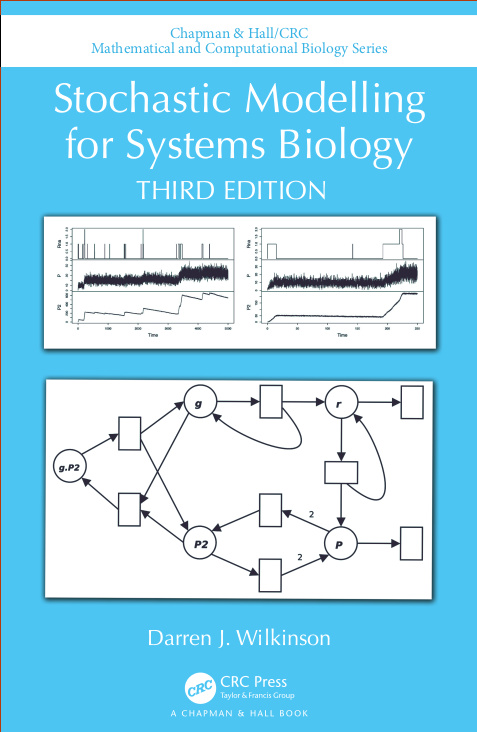
\includegraphics[height=\textheight]{cover-3e}}
}

\frame{
  \frametitle{SMfSB3e: New in the third edition}
  \begin{itemize}
\item New chapter on spatially extended systems, covering the spatial Gillespie algorithm for reaction diffusion master equation (RDME) models in 1- and 2-d, the next subvolume method, spatial CLE, scaling issues, etc.
\item Significantly expanded chapter on inference for stochastic kinetic models from data, covering approximate methods of inference (ABC), including ABC-SMC. The material relating to particle MCMC has also been improved and extended.
\item Updated R package, including code relating to all of the new material
\item New R package for parsing SBML models into simulatable stochastic Petri net models
\item New software library, written in Scala, replicating most of the functionality of the R packages in a fast, compiled, strongly typed, functional language
\end{itemize}
  }

\frame{
  \begin{minipage}{0.45\textwidth}
    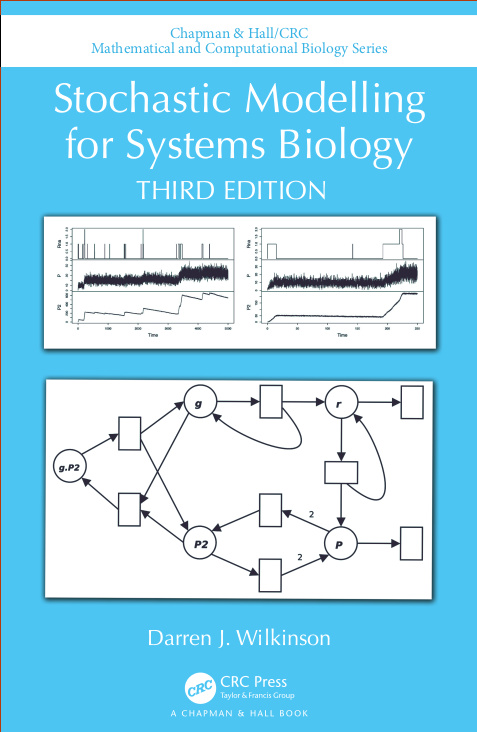
\includegraphics[height=0.8\textheight]{cover-3e}
  \end{minipage}
  \begin{minipage}{0.45\textwidth}
    \begin{itemize}
    \item In the press right now
    \item Published 29th November
      \item Pre-order now for Xmas!
      \item New website/GitHub repository
        \item Lots of new, improved and updated software --- all free, open source, well-documented and available now
    \end{itemize}
  \end{minipage}\\
  \vspace{1.5ex}
    \centerline{\alert{\url{https://github.com/darrenjw/smfsb}}}
  }



\end{document}

